\documentclass{MScthesisITEM}

% this package is just to generate text for demo-purposes
\usepackage{blindtext}
\usepackage{graphicx}
\usepackage{textcomp}
%\usepackage[table,xcdraw]{color}
%\usepackage[table]{xcolor}
\usepackage{lipsum}                     
\usepackage{xargs}                      
\usepackage{xcolor}
\usepackage{fancyvrb}
\usepackage{csquotes}
\usepackage{booktabs}
\usepackage{tabularx}
\usepackage{lipsum}
\usepackage{listings}

\usepackage[euler]{textgreek}
\usepackage[colorinlistoftodos,prependcaption,textsize=tiny]{todonotes}
\newcommandx{\unsure}[2][1=]{\todo[linecolor=red,backgroundcolor=red!25,bordercolor=red,#1]{#2}}
\newcommandx{\change}[2][1=]{\todo[linecolor=blue,backgroundcolor=blue!25,bordercolor=blue,#1]{#2}}
\newcommandx{\info}[2][1=]{\todo[linecolor=OliveGreen,backgroundcolor=OliveGreen!25,bordercolor=OliveGreen,#1]{#2}}
\newcommandx{\improvement}[2][1=]{\todo[linecolor=Plum,backgroundcolor=Plum!25,bordercolor=Plum,#1]{#2}}
\newcommandx{\thiswillnotshow}[2][1=]{\todo[disable,#1]{#2}}


%\graphicspath{/figs}
\graphicspath{ {/home/sindre/Documents/Master/MasterThesis/Latex/figs} }
\newcommand\tab[1][1cm]{\hspace*{#1}}

\usepackage{listings}
\usepackage{color}

\definecolor{dkgreen}{rgb}{0,0.6,0}
\definecolor{gray}{rgb}{0.5,0.5,0.5}
\definecolor{mauve}{rgb}{0.58,0,0.82}

\lstset{frame=tb,
  language=Java,
  aboveskip=3mm,
  belowskip=3mm,
  showstringspaces=false,
  columns=flexible,
  basicstyle={\small\ttfamily},
  numbers=none,
  numberstyle=\tiny\color{gray},
  keywordstyle=\color{blue},
  commentstyle=\color{dkgreen},
  stringstyle=\color{mauve},
  breaklines=true,
  breakatwhitespace=true,
  tabsize=3
}

\title{Understanding Data Analysis in an\newlinetitle End-to-End IoT System} % The title of your assignement; NB use \newlinetitle to start a newline
\author{Sindre Schei} % Your firstname and lastname
\professor{Frank Alexander Kraemer, ITEM} % Affiliation = ITEM for instance
\supervisor{David Palma, ITEM}

%% Uncomment the following in case you want subfigures; note that there will be a warning for the caption package
% \let\subcaption\undefined
% \let\subfloat\undefined
% \usepackage[bf]{caption}
% \usepackage{subcaption}

\DeclareGraphicsExtensions{.pdf,.jpg,.png}
%\graphicspath{{./figs/}}

\loadglsentries{glossary} 
\makeglossaries

\begin{document}
\selectlanguage{english}
\pagenumbering{roman}
\pagestyle{plain}
$lim_{n\to\infty}$

%% Only for the project; comment out the line below for the master's thesis; the front page will be generated automatically by DAIM
\titleITEM

%% Only for the master's thesis; for the project report the description is taken from It's Learning and added by the department
% \selectlanguage{english} % Change to 'norsk' if you are writing in Norwegian
% \begin{titlingpage}

\noindent
\begin{tabular}{@{}p{4cm}l}
\textbf{Title:} 	& Understanding Data Analysis in an \\& End-to-End IoT System\\
\textbf{Student:}	& \theauthor \\
\end{tabular}

\vspace{4ex}
\noindent\textbf{Problem description:}
\vspace{2ex}

\noindent The Internet of Things (IoT) is known as the concept of connecting everyday physical devices to the Internet. It is natural to assume that the popularity and development within this field will increase in the following years. This means that more and more things will be able to communicate over the Internet. In the process of developing IoT, an important part is to build reliable and scalable networks, and understanding where data should be processed concerning power consumptions and costs of transferring data in different parts of the network. 

\noindent The task of the thesis will be to access data in a complete prototype of an IoT network, and both collect and analyse the data. The goal is to study different alternatives for a typical IoT system and provide an overview of current state-of-the-art technologies, products and standards that can be used in such a setting. Data can be generated by using and comparing different sensors connected to end nodes in the network.

\noindent To achieve these goals, a central part will be to understand the benefits of processing data in the end nodes, concerning power, costs and time. This means much less data needs to be sent through the network. If the calculations needed are too complex, the measured data needs to be transferred to a central node with higher processing power and easier access of energy. Another part is testing devices and sensors needed, and write programming code associated with these. 

\vspace{6ex}

\noindent
\begin{tabular}{@{}p{4cm}l}
\textbf{Responsible professor:} 	& \theprofessor \\
\textbf{Supervisor:}			& \thesupervisor \\
\end{tabular}

\end{titlingpage}
% \cleardoublepage

%% There must be an abstract in English, even though the main text is in Norwegian
\selectlanguage{english}
%\pagestyle{empty}
\begin{abstract}


\noindent The \gls{iot} is known as the concept of connecting everyday physical devices to the Internet. It is natural to assume that the popularity and development within this field will increase in the following years. This means that more and more things will be able to communicate over the Internet. In the process of developing \gls{iot}, an important part is to build reliable and scalable networks, and understanding where data should be processed concerning power consumption and costs of transferring data in different parts of the network.

\noindent The task of the thesis will be to access data in a complete prototype of an \gls{iot} network, and both collect and analyse the data. The goal is to study different alternatives for a typical \gls{iot} system, and provide an overview of current state-of-the-art technologies, products and standards that can be used in such a setting. Data can be generated by using and comparing different sensors connected to end nodes in the network. A complete network of both \glspl{microcontroller} and \glspl{singleBoardComputer} will be built and explained in this thesis. The network will from now on be referred to as \textit{testbed}. 

\noindent \Glspl{microcontroller} as end nodes in an \gls{iot} network will be the central element tested in this thesis. The main focus is to establish a connection between two devices, A and B, and form a network between these that can transport data efficiently. A central point of discussion will be to find transfer protocols and technologies that can be used in such a network. It will be discussed the advantage and disadvantage of sending raw data, rather than doing computation in end nodes. The main focus will be on optimal throughput in the network. To do this, a deep understanding of the benefits of processing data in the end nodes, concerning power, costs and time is needed. 
%If the calculations needed in the network are too complex to be executed in an end node, the measured data needs to be transferred to a central node with higher processing power and easier access of energy. 

\noindent Results from this work include graphs and discussions explaining in which case the different transport protocols suggested are preferred, from tests done in the testbed. These show that different protocols are suited for different usage, and that one of the tested possibilities more stable than the other in the tests presented. Both protocols registered their highest measured \gls{goodput} at approximately 600 bytes/second. Being a quite slow transfer rate, this opened up for another discussion about the possible use cases for future \gls{ble}-based \gls{iot} applications. 

\noindent Keywords: Optimizing payload sizes, fragmentation, maximizing throughput, power usage. 


\end{abstract}
\cleardoublepage

%% Only for the master's thesis; if the main text is in English and you can write Norwegian, there must be an abstract in Norwegian as well.
\selectlanguage{norsk}
\pagestyle{empty}
\renewcommand{\abstractname}{Sammendrag}
\begin{abstract}
\noindent Tingenes Internet, mer kjent under det engelske navnet Internet of Things (IoT), er konseptet der hverdagslige fysiske gjenstander kobles til Internet. Det er naturlig å anta at populariteten og utviklingen rundt dette vil være økende de kommende årene. Dette betyr at flere og flere ting vil kunne kommunisere over Internet. I prosessen der Tingenes Internet utvikles, er en viktig del å bygge pålitelige og skalerbare nettverk, samt å forstå hvor i nettverket data bør prosesseres med tanke på energibruk og kostnader ved å overføre data mellom deler av nettverket. 

\noindent Hovedoppgaven presentert i denne avhandlingen vil være å jobbe med data i en komplett prototype av et Tingenes Internet-nettverk, og både samle og analysere dataene. Målet er å studere de forskjellige alternativene til et slikt nettverk, samt lage en oversikt over teknologiene og standardene som kan bli brukt i denne sammenhengen. Nødvendig data kan samles ved å sammenligne forskjellige sensorer koblet til endenodene i nettverket. Et komplett nettverk bestående av både mikrokontrollere og små datamaskiner på en brikke, vil bli bygget og forklart i denne oppgaven. Dette nettverket vil fra nå av refereres til som \textit{testbed}. 

\noindent Et sentralt testelement i denne oppgaven vil være bruk av mikrokontrollere som endenoder i et Tingene Internet-nettverk. Hovedfokuset er å sette opp en nettverksforbindelse mellom to enheter, A og B, og danne et nettverk mellom disse slik at data kan overføres på en effektiv måte. I diskusjonen vil et viktig punkt være å finne transportprotokoller og teknologier som kan benyttes i et slikt nettverk. Det vil bli diskutert fordelene og ulempene ved å transportere rådata istedenfor å gjøre utregninger i endenodene. Hovedpoenget her vil være gjennomstrømmingen av data i nettverket. For å gjøre dette trengs en dyp forståelse av fordelene ved å prosessere data i endenodene med tanke på energi, kostnader og tid. 

\noindent Resultatene fra arbeidet består av grafer og diskusjoner rundt disse for å forklare i hvilke situasjoner de forskjellige protokollene som har blitt testedt er foretrukket. Utgangspuntket er tester gjort i testbed. Disse testene viser at de forskjellige protokollene egner seg i ulike situasjoner, men at en av de er mer stabil enn den andre protokollen som denne avhandlingen presenterer. Begge protokollene hadde høyest målte \textit{gls{goodput}} på omkring 600 bytes/sekund. Siden dette er en forholdsvis lav sendingsrate åpnet dette for en annen diskusjon om mulig bruk i fremtidige Tingenes Internett-nettverk der lavenergi Bluetooth er benyttet.

\noindent Nøkkelord: Optimalisering av størrelser på faktiske data, fragmentering av datapakker, maksimere pakkegjennomstrømning, energiforbruk. 


  
\end{abstract}
\cleardoublepage

\selectlanguage{english}% Change to 'norsk' if you are writing in Norwegian

\renewcommand{\abstractname}{Preface}
\begin{abstract}

This thesis was issued by the Department of Telematics (ITEM) at the Norwegian University of Science and Technology (NTNU) the spring of 2016 as a Master Thesis in Telematics. 
The responsible professor has been Frank Alexander Kraemer, ITEM, who has given
helpful advice on how to build up and write such a large project, as
well as answering questions and providing support the whole period. David Palma has been the supervisor, giving impressively close monitoring of the project to fill in ideas, thoughts and good advice to help me finish the thesis. I would like to thank both these ITEM representatives for the work they have put down to make this project as good as possible. 

Secondly, I would like to thank fellow students for the many discussions, good advice and other more social activities the last five years. I would like to point out the guys at A-179 for their support, Jon Anders for helping me with code specific problems during the programming period, and Anders for the many hours we spent together setting up central parts of the network described in this thesis. Special thanks to you!

Last, but not least, I would like to thank my family for their support both during the period of this thesis, but also during my entire period as a student. Special thanks to my father, Svenn Arne, for helping me review the thesis and to get a discussion point with someone without a technical background. 



\end{abstract}
\cleardoublepage

% similarly you may add a separate acknowledgments page

\tableofcontents*
\cleardoublepage

%% include if relevant
\listoffigures
\cleardoublepage

%% include if relevant
\listoftables
\cleardoublepage

%% include if relevant
%\listofalgorithms
%\addcontentsline{toc}{chapter}{List of Algorithms}
%\cleardoublepage


%% include if relevant
\printglossary[title=List of Acronyms,type=\acronymtype] % prints just the list of acronyms
\cleardoublepage

%% include if relevant
\printglossary[title=Glossary, style=long]
\cleardoublepage
\glsaddall[]

\pagenumbering{arabic}
\pagestyle{ruled}
%\chapter{Example}
\label{chp:example} 

Here is an example of how to use acronyms such as \gls{ntnu}. The second time only \gls{ntnu} is shown and if there were several you would write \glspl{ntnu}. And here is an example\footnote{A footnote} of citation~\cite{Author:year:XYZ}. 

\Blindtext[3][1]

\begin{figure}
\centering
% dummy figure replacement 
\begin{tabular}{@{}c@{}}
\rule{.5\textwidth}{.5\textwidth} \\
\end{tabular}
\caption{\label{fig:example}A figure}
\end{figure}

\section{First section}\label{sec:first_section}

\subsection{First subsection with some \texorpdfstring{$\mathcal{M}ath$}{Math} symbol}\label{sec:first_ssection}

\blindtext
\begin{itemize}[topsep=-1em,parsep=0em,itemsep=0em] % see http://mirror.ctan.org/macros/latex/contrib/enumitem/enumitem.pdf for details about the parameters
 \item item1
 \item item2
 \item ...
\end{itemize}

\subsection{Mathematics}

\blindmathtrue
\blindtext

\begin{proposition}\label{def:a_proposition}
A proposition... (similar environments include: theorem, corrolary, conjecture, lemma)

\end{proposition}

\begin{proof}
\vspace*{-1em} % Adjust the space when parskip is set to 1em
And its proof.
\end{proof}

\begin{table}
\caption{\label{tab:example}A table}
\centering
\begin{tabular}[b]{| c | c | c | c | c |}
\hline
a & b & c & d & e \\ \hline
f & g & h & i & j \\ \hline
k & l & m & n & o \\ \hline
p & q & r & s & t \\ \hline
u & v & w & x & y \\ \hline
z & æ & ø & å &   \\ \hline
\end{tabular} 
\end{table}

\subsection{Source code example}

% \floatname{algorithm}{Source code} % if you want to rename 'Algorithm' to 'Source code'
\begin{algorithm}[h]
  \caption{The Hello World! program in Java.}
  \label{hello_world}
  % alternatively you may use algorithmic, or lstlisting from the listings package
  \begin{verbatim}
  
class HelloWorldApp {
  public static void main(String[] args) {
    //Display the string
    System.out.println("Hello World!");
  }
}
\end{verbatim}
\end{algorithm}

You can refer to figures using the predefined command like \fref{fig:example}, to pages like \pref{fig:example}, to tables like \tref{tab:example}, to chapters like \Cref{chp:example} and to sections like \Sref{sec:first_section} and you may define similar commands to refer to proposition, algorithms etc.

%% include here the other chapters

\chapter{Introduction}
\label{chp:introduction} 


\section{Motivation}

Internet of Things (IoT) 



is known as the concept of connecting everyday physical devices to the Internet. It is natural to assume that the popularity and development within this field will increase in the following years. This means that more and more things will be able to communicate over the Internet. In the process of developing IoT, an important part is to build reliable and scalable networks, and understanding where data should be processed concerning power consumptions and costs of transfering data in different parts of the network.

\section{Methodology}

\section{Scope and Objectives}

\subsection{Scope}

\subsection{Objectives}

\noindent \textbf{O.1: Build a star network of microcontrollers}

\noindent\textbf{O.2: Connect sensors to the end-nodes to collect data}

\noindent\textbf{O.3: Gather information of the data sent through the network}

\noindent\textbf{O.4: Analyse and discuss the gathered information}

\section{Structure}

\chapter{Background}
\label{chp:background} 

This thesis describes the setup and usage of an End-to-End \gls{iot} system. In order for this to be set up by others later to perform reproducible tests, a detailed description of components, sensors and protocols used is needed. This chapter will go through the background information of the devices, technologies and protocols used, and why these where chosen over other alternatives. 

%\section{Internet of Things} % Tjae

%Comment: Read Future Internet: The Internet of Things from 2010.  \cite{gubbi2013internet}

%Comment: Read http://ac.els-cdn.com/S1570870512000674/1-s2.0-S1570870512000674-main.pdf?_tid=6f15526e-eae8-11e5-addc-00000aab0f6b&acdnat=1458072152_0740a71f559cd8ae1ebd0ce4a687e122

%M2M and "M2T" ("Machine to Thing-communication"). Classification of a thing? \cite{tan2010future}. 

%\section{Challenges}


\section{Bluetooth Low Energy (Bluetooth Smart)}

%Read this:

\gls{ble} is a wireless technology for short range communication developed by the Bluetooth Special Interest Group \cite{gomez2012overview}. The idea was to create a low energy single-hop network solution for \glspl{pan}. A major advantage of this is that Bluetooth 4.0 is already a well established technology in cell phones, laptops and several other devices, and \gls{ble} can use several similarities with this. The 6LoWPAN Working Group has recognized the importance if \gls{ble} in \gls{iot} \cite{hui2008extending}.

The protocol stack of \gls{ble} has two main parts, the controller and the host. In the system used in this thesis this represents the Raspberry Pi as the controller (master) and Nordic nRF52 as the host (slave). The communication between these is done through the standard \gls{hci}. All slaves are in sleep mode by default, and are woken up by the master when communication is needed. Links are being identified by a randomly generated 32-bit code. 

In the case of the network used in this thesis, when the \gls{ble} slave has been connected to a master, it stops searching for other masters, and it is not possible to connect to several masters. This means that we are only able to create a \textit{star network}, not a \textit{mesh network}. This could possibly be an idea for improvement later. Other than this, \gls{ble} seems like a very good alternative in this project. 



Check out: Mikhail Galeev - BLE

\subsection{\gls{hci}}

\subsection{ACL}

\section{6LoWPAN}

%To identify sensors and devices in low energy sensor and device networks, a new protocol was needed. 

\gls{6lowpan} is a defined protocol for using \gls{ipv6} in low enerdy networks, to identify sensors and devices, as defined in the IEEE 802.15.4. 

To use the Internet Protocol was proposed by Geoff Mulligan and the 6LoWPAN Working Group in \cite{mulligan20076lowpan}. In this paper the advantage of \gls{6lowpan} is explained as the easiest way to use standard protocols such as \gls{udp}, \gls{tcp}, \gls{icmp}, gls{dns} and \gls{tftp}, since they can be used directly without the requirement of a translation mechanism. They are already adapted to run over \gls{ipv6}. 

In addition to this, the paper argues that \gls{6lowpan} was developed to be used in small sensor networks. Implementations can fit into 32Kb flash memory parts, wich is smaller than Zigbee and Zensys (which is the two main comparisons made in the paper). It also uses an impressive header comparison mechanism that allows the transmission of \gls{ipv6} packets in 4 bytes, much less than the standard 40 bytes. This is done by using stacked headers, same as in the \gls{ipv6} model, rather than defining a specific header as for \gls{ipv4}. This means that a device can send only the required part of the stack header, and does not need to include header fields for networking and fragmentation \cite{hui2008extending}. 

\gls{6lowpan} was therefore a natural tool to use in this project, in the \gls{ipv6} and \gls{ble} based network. 

%The \gls{6lowpan} architecture was developed to allow \gls{ipv6} packets to be sent over low energy networks.  

\section{Raspberry Pi}

Developed by Element 14, the Raspberry Pi has become a central tool for many people wanting to get started using microcomputers. This was therefore a natural starting point for us as well. 

\begin{figure}[ht]
    \centering
    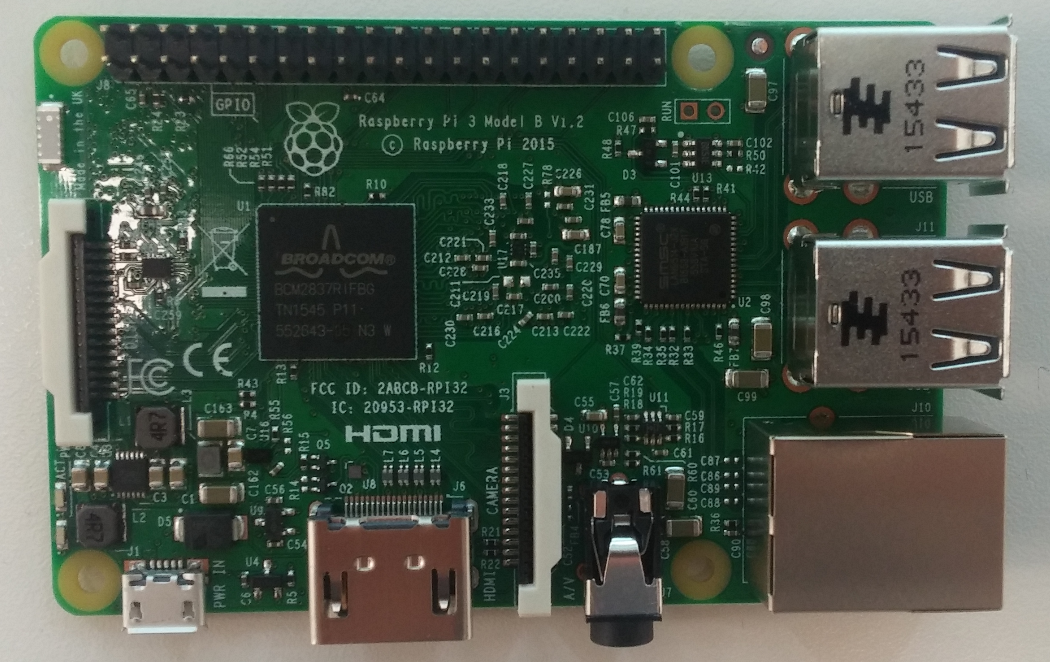
\includegraphics[scale=0.35]{pi3.png}    
    \caption{Raspberry Pi 3}
    \label{fig:piPicture}
\end{figure}



The Raspberry Pi 2 model B+ is the second generation of its kind, and its \textit{ARMv7 processor} has approximately six times the performance of the predecessor \cite{raspberryPi2}. With a USB Bluetooth dongle connected, it is quite simple to enable both \gls{6lowpan} and \gls{ble}, given that the right Unix kernel has been used in the \gls{os} of the Pi.

Later in this thesis, the processing power of the Pi compared to performing calculations in the end-points will be a central topic for discussion. 

\subsection{Ubuntu Mate}

Along with the Raspberry Pi, we needed a good and stable operating system with a kernel that supported the \gls{6lowpan} architecture. For this, Ubuntu Mate version 15.10 with kernel version 4.15 was chosen, and used on the Raspberry Pi. As other versions of Ubuntu this is Unix based, and has a complete \gls{gui} of a full \gls{os}. 

\section{nRF52}

The nRF52 is developed by Nordic Semiconductor, and is being described as a family of highly flexible, multi-protocol system on chip. 

% Kok 

\begin{figure}[ht]
    \centering
    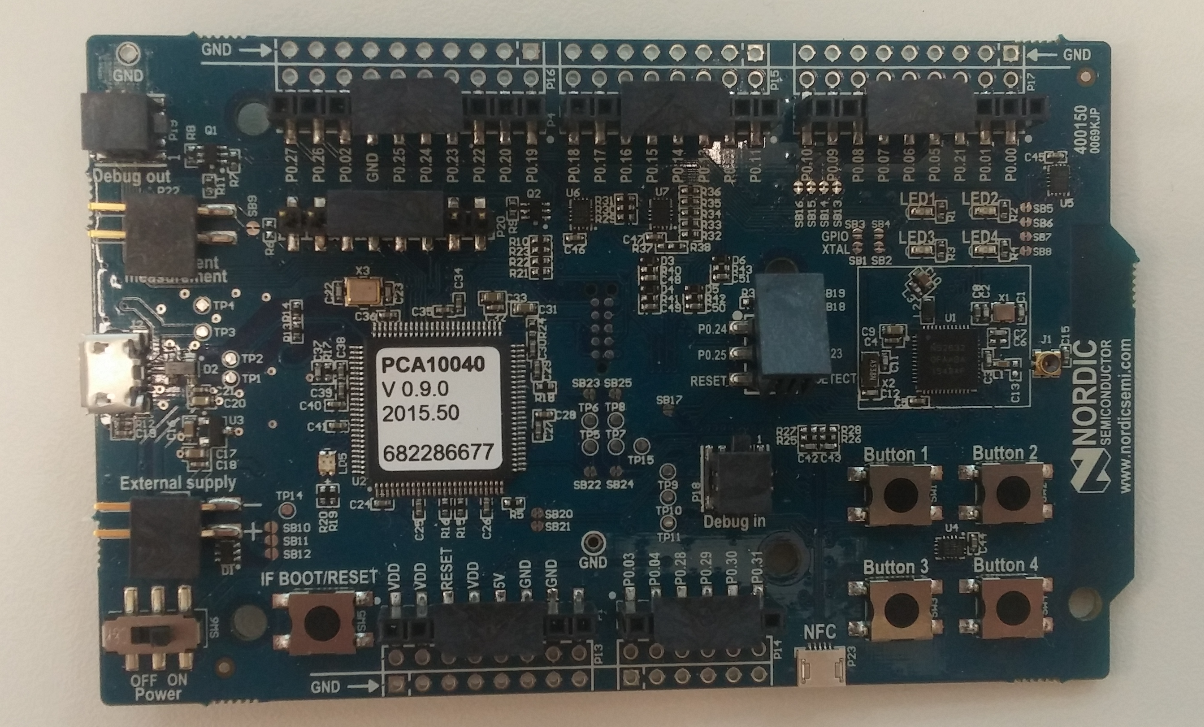
\includegraphics[scale=0.32]{nrf52.png}    
    \caption{Nordic Semiconductor NRF52}
    \label{fig:nrf52picture}
\end{figure}

\cite{nrf52Nordic}

Running at 64MHz it racks up impressive stats: EEMBC Coremark® score of 215 and 58 Coremark®/mA. Built in a cutting edge 55nm process technology the nRF52 Series is architected for todays need for speed, speed to carry out increasingly complex tasks in the shortest possible time and return to sleep, conserving precious battery power. Introducing a Cortex-M4F processor at its heart, it is the most capable Bluetooth Smart SoC on the market today.	
With a brand new multiprotocol radio architecture limits are pushed even further for Bluetooth Smart: A total link budget of 100dBm, -96dBm sensitivity, +4dBm output power and -42dBm selectivity, it is built to exist reliably and effectively in a busy 2.4GHz band. Couple this RF resilience with outstanding power consumption: 5.3mA at 0dBm TX output power and 5.4mA RX it is miserly with power when getting things done on-air.

 

Designed with wealth of digital and analog interfaces and peripherals, there’s something to cover every design requirement. The demands of today’s Bluetooth smart single chip designs are increasingly varied and complex, they can range from digital audio processing, to FFT/FIR and security algorithms, to driving device displays and UIs. Whatever the task, nRF52 series has it covered.

 

We’ve truly made low power easy. We haven’t just just great datasheet numbers, but an automatic and adaptive power management system which combined with extensive EasyDMA and PPI makes the nRF52 Series positively frugal with power.

 

nRF52 Series brings NFC for the first time to a Bluetooth Smart SoC. The on-chip NFC-A tag allows developers to take advantage of NFC ‘touch-to-pair’ functionality in their designs.

 

Maintaining the total flexibility philosophy of the nRF51 Series, it is a flash device. With 512kB flash + 64kB RAM on chip, developers keep all the software stack flexibility and Over-The-Air Device Firmware Upgrade (OTA-DFU) features they enjoyed with the nRF51 Series.

 

We understand that in the world of wearables, size really is everything, so we built a device that is the smallest Bluetooth Smart SoC to date measuring as small as 3.0 x 3.2mm (CSP). With an on-chip balun and a minimum of external components it has the smallest design footprint out there.

 

Tomorrow’s Bluetooth Smart Solutions are going to ask a lot. The nRF52 Series delivers.

% Kok slutt


% https://www.nordicsemi.com/Products/nRF52-Series-SoC

\subsection{Softdevice}




\section{Adafruit ADXL345 Accelerometer}

In order to do collect data, a sensor needed to be connected to the Nordic Semiconductor nRF52. The main thought behind the thesis was to measure vibrations, and a good accelerometer was needed. The Adafruit ADXL345 accelerometer was chosen for several reasons. 

\begin{itemize}
  \item It is the same accelerometer built in on the Zolertia Z1 microcontroller
  \item It can measure acceleration in all three axes, X, Y and Z.
  \item It sends digital data right away. This means there is no need to use computational power to calculate digital values as needed if the data was captured by an analog accelerometer. 
  \item It supports both \gls{i2c} and \gls{spi}, which makes it easy to connect to the nRF52. 
\end{itemize}


\begin{figure}[ht]
    \centering
    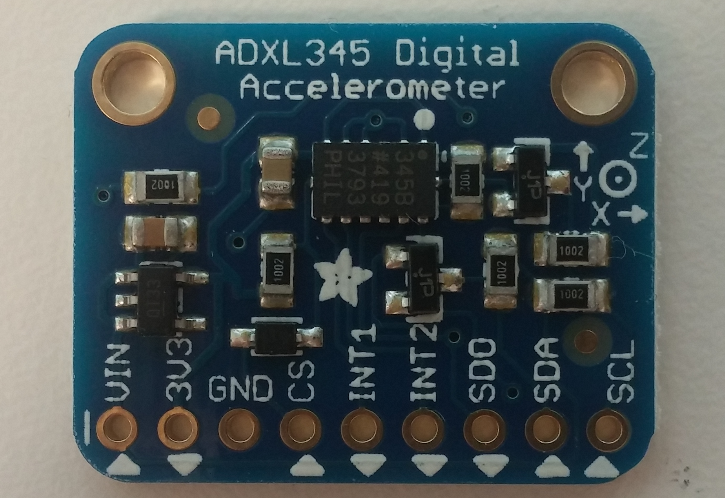
\includegraphics[scale=0.32]{ADXL345.png}    \caption{ADXL345 Accelerometer}
    \label{fig:adxl345}
\end{figure}

\newpage

\section{Transport protocols}

\subsection{Network layers}

\subsection{\gls{coap}}

%The \\ protocol is described in the documentation as follows: 

\gls{coap} is a transport protocol designed to be used in constrained networks for \gls{m2m} communication. It is \gls{udp} based, and works good in low-power and lossy networks. It can be used with microcontrollers, and with \gls{ipv6} and \gls{6lowpan}. Both GET and PUSH functionality can be used, as well as \textit{observable} GET. This means that a server can "subscribe" to end notes in the network, and get updates either after a given timespan or when changes have been made. This therefore looked like a promising protocol to use, and was chosen as the first transport protocol to test the network \cite{shelby2014constrained}.
 



\subsection{\gls{mqtt}}

Another transport protocol that could be used in such a network of microcontrollers is \gls{mqtt}. This is  known as a publish-subscribe based on \gls{tcp}, using a \gls{mqtt} broker. \gls{ntnu} does have a broker that is possible to use, or a broker can be rented from several other places. Here a 

\cite{hunkeler2008mqtt}

\subsection{\gls{radvd}}


\section{Software tools}

As \gls{ide}, the \textit{KEIL Vision} was used, as recommended by Nordic Semiconductor (where?), for writing C programming. For other programming languages (for instance Python 3.4, HTML, CSS, JavaScript, Flask and AJAX) \textit{Sublime Text 2} for Windows and Linux was used, as well as \textit{Pluma} for Ubuntu Mate on the Raspberry Pi. 

\subsection{Other}

Wireshark, Firefox, GitHub







\chapter{System Architecture}
\label{chp:architecture} 

The purpose of this thesis is to build an end-to-end system, to be able to transfer data all the way from sensors connected to a microcontroller to a server. This chapter will describe in detail how the different components of the system has been connected together, and how the different protocols has been configured to read and transfer data efficiently. 


\begin{figure}[ht]
    \centering
    \includegraphics[scale=0.7]{MasterArchitecture2.png}    
    \caption{System architecture}
    \label{fig:systemArchitecture}
\end{figure}

Figure \ref{fig:systemArchitecture} shows how the complete end-to-end system of this thesis is set up. In short terms, the \textit{Nordic Semiconductor nRF52} is connected to a  \textit{Raspberry Pi 3} using \gls{6lowpan} and \gls{ble}. This means that they are able to communicate using \gls{ipv6} addresses, even though the nRF52 only has a bluetooth antenna built in, as shown in figure \ref{fig:nrf52chipDetail}. The limitations of \gls{ble} means that the nRF52 can only connect to \textit{one} device at the time. Several of these put together are therefore forming a \textit{star network} using the \textit{Raspberry Pi} as a central point of connection. Computations can now either be done in the end nodes at the \textit{nRF52s}, at the \textit{Raspberry Pi}, or forwarded to a web server or another computer with more computational power. Data can also be displayed directly to a web page from the \textit{Raspberry Pi}. 
 
%\newpage

There are in general three main limitations in a network such as this:

\renewcommand{\labelitemi}{$\textasteriskcentered$}
\begin{itemize}
  \item Computational power in the different nodes
  \item Battery capacity of the end nodes
  \item Network limitations between the nodes
\end{itemize}

A central part of the testing in this thesis will be to test the different limitations, and to understand the pros and cons of doing computations in end nodes, compared to transferring information to a server with \textit{much} more computational power. Power usage is very often closely related to computational power, and will also be a central factor. The next section will contain a walk-through of the system, from the smallest to the biggest component, to explain their computational and power capabilities, and how they can communicate efficiently. 

Computational power is closely related to power usage. The nRF52 microcontroller is battery powered using a small \textit{3V Lithium CR 2032} battery. Given this limitation the computational power will be limited as well. The optimal solutions therefore seems to handle as little data as possible here. 


\section{Connecting Raspberry Pi and nRF52}


%As a microcontroller the nRF52 works good in this network, both as a low-power and powerful device. 

To set up the communication between a Raspberry Pi and the nRF52, the two code examples TWI and Observable server from Nordic Semiconductor was used as a starting point for coding on the nRF52. It was however quite tricky to set connect these two together the first time. The following recipe is what worked best. 

Install an \gls{os} on the Raspberry Pi that has a Linux kernel version later than 3.18. On \textit{Raspbian} version 3.18 is the only stable (Note: Jan. 2016), but \textit{Ubuntu Mate} is stable in version 4.15. \textit{Ubuntu Mate} was therefore chosen as the best and most stable \gls{os}. When this is done a resizing of the file system is needed to use all the capacity of the memory card. This is not necessary, but recommended to be able to use more than 4GB of the memory card. To resize, run the following commands

\begin{verbatim}
sudo fdisk /dev/mmcblk0
\end{verbatim}

Delete partition (d,2), and run the following after a reboot

\begin{verbatim}
sudo resize2fs /dev/mmcblk0p2
\end{verbatim}

To use \gls{ble}, install Bluez and radvd using \textit{apt-get} in a \textit{Unix terminal}:

\begin{verbatim}
apt-get install radvd wireshark bluez
apt-get upgrade
apt-get update
\end{verbatim}
%\end{lstlisting}

To activate \gls{ipv6} forwarding, uncomment the following line (remove "\#") in the file \textit{etc/sysctl.conf}

\begin{verbatim}
net.ipv6.conf.all.forwarding=1
\end{verbatim}

Add the \textit{bt0 interface} in \textit{radvd.conf}:

\begin{verbatim}
touch /etc/radvd.conf
pico /etc/radvd.conf
\end{verbatim} 

Write in the bt0 interface

\begin{verbatim}
interface bt0
{
    AdvSendAdvert on;
    prefix 2001::/64
    {
        AdvOnLink off;
        AdvAutonomous on;
        AdvRouterAddr on;
    };
};
\end{verbatim} 

To mount the modules \textit{bluetooth\_6lowpan, 6lowpan and radvd}, add the following to \textit{/etc/modules}. 

\begin{verbatim}
bluetooth_6lowpan
6lowpan
radvd
\end{verbatim}

It is now possible to use the \textit{hcitool} command. 

\begin{verbatim}
hcitool lescan
\end{verbatim}

This command will scan for \gls{ble} devices nearby, and find the bluetooth address, for instance \textit{0211:22FF:FE33:4455}. The normal procedure in this case would be to run the following command: 

\begin{verbatim}
echo 1 > /sys/kernel/debug/bluetooth/6lowpan_enable
hcitool lecc 0211:22FF:FE33:4455
service radvd restart
\end{verbatim}

This command never established a stable connection in this system. It was not possible to test the connection, and each connected device became automatically disconnected after about 15 seconds. The reason for this was never found. Instead it was possible to not use \textit{hcitool} for this part, and the following commands worked fine:

\begin{verbatim}
echo 1 > /sys/kernel/debug/bluetooth/6lowpan_enable
echo "connect 0211:22FF:FE33:4455 1" > /sys/kernel/
debug/bluetooth/6lowpan_control
service radvd restart
\end{verbatim} 
\todo{FIX verbatim new line? }

The command \textit{hcitool con} shows the connected \gls{ble} devices. If the device is connected, the connection can be tested by typing:

\begin{verbatim}
ping6 2001::0211:22FF:FE33:4455
\end{verbatim}


Using the basic examples provided by Nordic Semiconductor described in chapter \ref{chp:architecture}.3, it was now possible to send messages both using \gls{coap} \gls{con} and \gls{non}.  


\section{Connecting nRF52 and ADXL345}

\todo{Can possibly write much more here, code samples in appendix, things that needed to be changed and so on}

The ADXL345 Accelerometer used was connected using \gls{i2c}, which is quite straight forward using the nRF52. Connection scheme is as follows (nRF52 -> ADXL345): 

\begin{itemize}
  \item 5V -- VIN		\tab  	\textit{Power source, \textbf{\textcolor{green}{green cable}} in Figure \ref{fig:nrf-adxl345}}
  \item GND -- GND 		\tab 	\textit{Ground, \textbf{\textcolor{red}{red cable}} in Figure \ref{fig:nrf-adxl345}}
  \item P0.27 -- SDA	\tab	\textit{\gls{i2c} Serial Data Line, \textbf{\textcolor{orange}{orange cable}} in Figure \ref{fig:nrf-adxl345}}
  \item P0.26 -- SCL	\tab 	\textit{\gls{i2c} Serial Clock Line, \textbf{\textcolor{brown}{brown cable}} in Figure \ref{fig:nrf-adxl345}}
\end{itemize} 

\begin{figure}[ht]
    \centering
    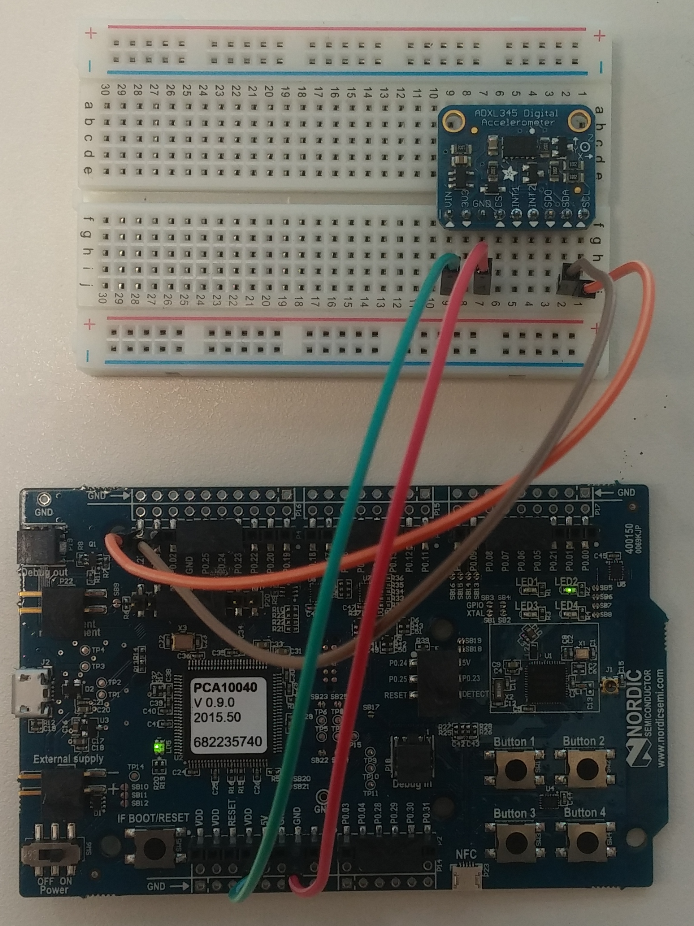
\includegraphics[scale=0.35]{nrf-adxl.png}    \caption{Connected nRF52 -- ADXL345}
    \label{fig:nrf-adxl345}
\end{figure}

After this is done it is possible to write to and read from the registers of the accelerometer over the two SDA and SCL cables. 


\subsection{Connection challenges}

Following instructions from a representative from Nordic Semiconductor, the bt0 interface was set up using the recommended \gls{ipv6} prefix: \textit{2001:bt8::1/64} in in the file \textit{etc/sysctrl.conf}, and after that trying to connect and test the connected devices using addresses on the form: 

\begin{verbatim}
ping6 2001:bt8::0211:22FF:FE33:4455
\end{verbatim}

This turned out not to work on the \gls{ipv6} network used on \gls{ntnu}, where the standard prefix is \textit{2001::1/64}, without the \textit{db8}. Both solutions should however work in other \gls{ipv6} networks. 

\subsection{bt8}

\todo{Descibe bt8-problem and devzone.nordicsemi.com and infocenter.nordicsemi.com}

\todo{Describe why I dropped the accelerometer}



\section{Nordic Semiconductor example code}

Nordic Semiconductor has provided several examples along with the nRF52-DK documentation, that can be used as a starting point when programming applications to the device. These files are written in the programming language \textit{C}. 

\subsection{\gls{coap}}

As a first step, the nRF52 needed to communicate with the Raspberry Pi. As explained in section 2.6, a good starting point for this is to use the \gls{coap} trasnport protocol, and the example of the use of this on the device. The \textit{CoAP Server} and \textit{CoAP Observer} was loaded into two different nRF52 devices, and both of them connected to the Raspberry Pi. Now \gls{radvd} had to be activated on the Pi, to be able to use this as a \textit{forwarding server}. 

\begin{figure}[ht]
    \centering
    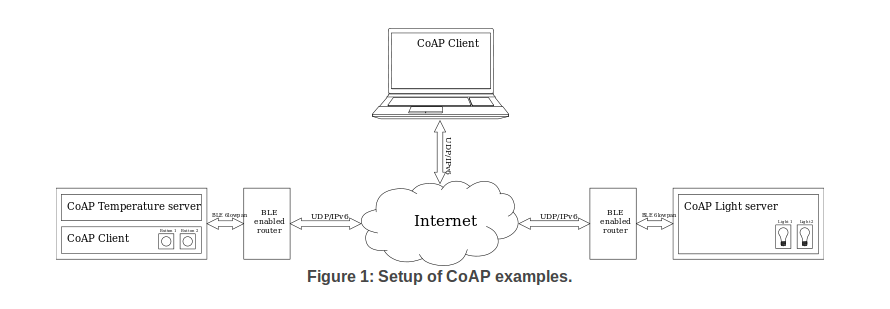
\includegraphics[scale=0.47]{CoAPExample.png}    
    \caption{CoAP Client-Server communication example}
    \label{fig:CoAPexample1}
\end{figure}
\todo{Remove "Figure 1" from image}

Figure \ref{fig:CoAPexample1} shows the initial CoAP example, by using two nRF52 devices, \gls{ble} over \gls{6lowpan} and a \gls{ble} enabled router (Raspberry Pi) on both ends in this case. As the figure \ref{fig:CoAPexample1} shows, the code example for the \gls{coap} client includes two different cases: 

\begin{itemize}
  \item In the fist case the \gls{coap} client acts as a client requesting services from the \gls{coap} server. Button 1 and 2 will control light 1 and 2 on the nRF52 server, which will send a conformation back if the light was changed or if something went wrong.
  \item In the second case the \gls{coap} server is excluded, but the \gls{coap} client works as a server that can handle requests from the router. In this case it is possible to use \textit{Copper} in a \textit{Firefox browser} on the Raspberry Pi to act as a client to request values from a simulated temperature sensor on the server. The server will  then send the current simulated temperature back, or tell if something went wrong. 
\end{itemize} 

Figure \ref{fig:CoAPexample1} shows the capture of packets using Wireshark. 

\begin{figure}[ht]
    \centering
    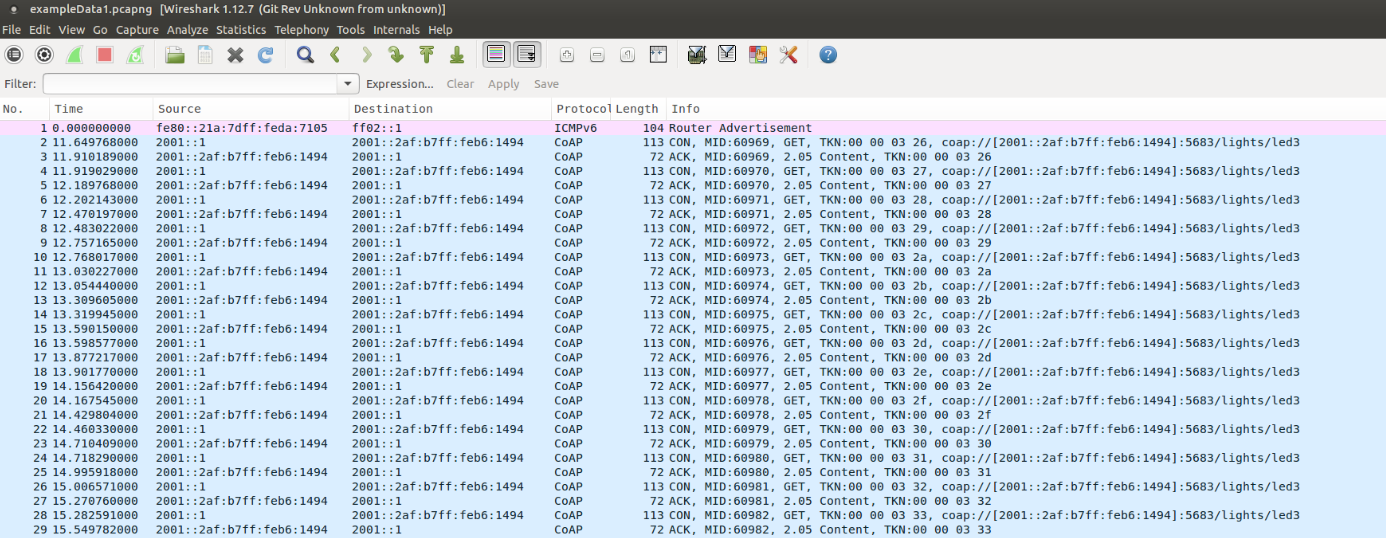
\includegraphics[scale=0.27]{CoapEx1captureCropped2.png}    
    \caption{CoAP Client-Server example Wireshark capture}
    \label{fig:CoAPexample1}
\end{figure}


This gives us the sequence diagram shown in Figure \ref{fig:seq1}. 

\begin{figure}[ht]
    \centering
    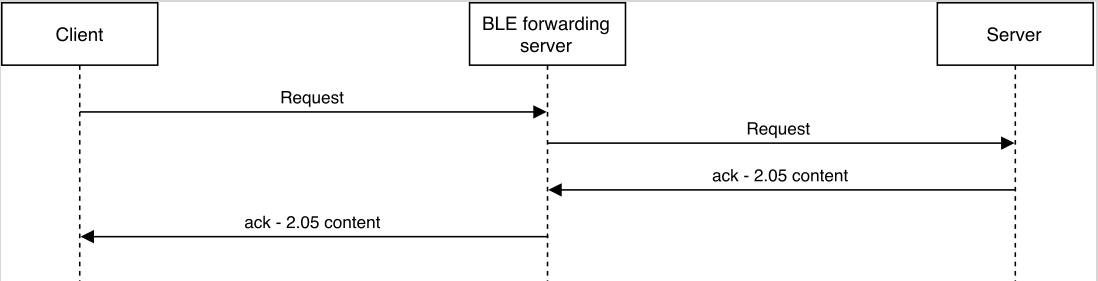
\includegraphics[scale=0.27]{seq1.png}    
    \caption{Sequence diagram CoAP Client-Server example}
    \label{fig:seq1}
\end{figure}

\todo{Create new sequence diagram}

This works fine, and by writing a Python script running on the \textit{Raspberry Pi} it is possible to request data by \textit{GET messages} as soon as the \textit{nRF52} is ready. However, as shown in figure \ref{fig:pingComparison} and figure \ref{fig:ping2}, the network transfer rate can vary a lot. The limitations in \gls{ble} and \gls{6lowpan} makes this much slower than a standard \gls{ipv6} connection, and the \textit{ping} \gls{rtt} varies from 100 ms all the way up to over 600 ms. As a comparison, to \textit{ping google.com} from the same Raspberry Pi using \gls{ipv6} takes on average 15 ms. A comparison of this is shown in figure \ref{fig:pingComparison}. This is therefore a clear limitation of sending rate in the system. Because of this, the maximum transfer rate achieved in the system using the standard \gls{coap} server example is one message every 200 ms. 

Using the standard \gls{coap}, described as \textit{CoAP CON} in this thesis, messages are sent with a "\gls{tcp} mindset". This means that every message sent by the client must receive an \gls {ack}. This is very stable, and ensures that every message gets to its destination, but it requires a lot of unnecessary computational power in the leaf node in systems where the importance of each message is not that high. The system is meant to be used with tools for analysing, and it is not essential that data needs to get to its destination right away. In these cases there is another alternative, known in this thesis as \textit{CoAP NON}. This is more like a "\textit{gls{udp} mindset}", where each packet does \textit{not} need an \gls{ack}. This halves the number of packages sent, saves a lot of the network as well as actions needed to be done by the nRF52 where power consumption is a huge issue. Therefore the \textit{\gls{coap} Observable} function looked very interesting, and will therefore be directly compared to \textit{standard gls{coap}} later in this thesis.   

%To improve this, the best solution is to either 

%This works fine, but in the case of the system built in this thesis there is no need to receive a confirmation for every single message.  It therefore makes sense to send messages in an \textit{\gls{udp} fashion}, where packages are being sent right away without acknowledgement. .   

\subsection{Observable \gls{coap}}

In the given Nordic example of a \gls{coap} observable server, the problem of unnecessary packets being sent can be resolved. Using this it is easy to set up a server that can be observed by either a nRF52 client or a \gls{ble} forwarding server. The observable end point sends a \textit{CON-ACK request} in a given time interval to assure that the observing client is still there. As long as this message is being responded the server will continue to send data without any requirements of an \gls{ack}. 

\begin{figure}[ht]
    \centering
    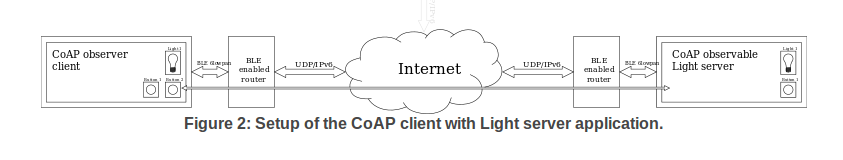
\includegraphics[scale=0.47]{CoAPObservalbFigure2.png}    
    \caption{CoAP Observable Server example}
    \label{fig:CoAPexample2}
\end{figure}
\todo{Remove "Figure 1" from image}



\todo{Create new sequence diagram for Observable as well}


\section{Getting acceleration values}

As soon as the sending of values is being handled in a good way, the next step is to read acceleration values from the ADXL345 accelerometer, which is connected to the NRF52 using the \gls{i2c} interface. 

Acceleration values can only be read from the ADXL345 if this has been correctly initialized at compile time. In order to do this, code to write to and read from the registers had to be added. The initializing process is described in the accelerometer data sheet \cite{adxlDataSheet}. In short, registers for \textit{data format control, initial power saving, interrupt enable control} and \textit{the offset of each axis} has to be written to in that order before the acceleration value from the different axes can be read.  

In the solution proposed in this thesis the acceleration values are being read as often as possible, limited by the processing power of the nRF52, and then stores in a simple dynamical char array before being sent and reset after one second. This turned out to be very time consuming and hard to solve in a good way, both because of problems with initializing the accelerometer correctly and making the nRF52 read and store the values fast enough to get proper data. The ideal solution would be to read at least 1000 values every second, to get a good starting point before analysing values. Neither the nRF52 or the ADXL345 turns out to be fast enough to do this in the implemented solution.  To not loose too much time on hardware problems, it was decided to focus more on analysing the data sent over the network communication with random generated data. 

Since the network connection between the nRF52 and Raspberry Pi was already stable, it was easy to generate random values of fixed length to send on the nRF52, and do measurements to calculate the optimal throughput between these two. The next chapter will therefore describe the data analysis of the data sent through this network in detail, and how to optimize the percentage of usable data being transported.  

\todo{Describe why not to gather acceleration values in this project}


\section{From Raspberry Pi to Network Computer or Server}

When running the Unix based \gls{os} Ubuntu Mate, the raspberry Pi can be used more or less as a regular computer. This has a pre-installed version of the most basic programs needed, for instance \textit{Mozilla Firefox Browser}, \textit{Pluma text editor} and \textit{Unix terminal}. This means that the user has several options on how to process data on this device: 

\begin{itemize}
  \item No computation: All data arrives as useful data, and can be posted directly to a web page or a server for storage
  \item No computation: Forward all data directly to a computer with more computational power
  \item Some computation: Analyse the data to find data that is not relevant to filter out
  \item Full computation: Do a full analyse of the data. The results can then be posted directly to a server or displayed on a web page. 
\end{itemize}

Which of these four options that is most relevant depends on the data, and how computational power is needed. It is possible to run the Raspberry Pi from a power bank, but this has not been tested in this project. When set up without a battery as power source, the Pi is the first node that could possibly do computations without having to take power limitations as a great concern. The main limitation is therefore computational power, while the main limitation may be battery power on the nRF52. It therefore makes sense to do some easy computation on this device. For instance, if this network is being used to measure vibrations, it is reasonable to assume about 1000 acceleration values every second, which represents a measuring rate of 1 kHz. It would then be perfectly reasonable to assume that the Pi could go through these values, and calculate whether or not the current acceleration value has breached a given threshold. This result can then be displayed directly on a web page or a connected monitor from the Pi. If however the system is to calculate \textit{patterns} in the acceleration values several values needs to be compared together. The need of complex algorithms to find these patterns is expected, before the results can be displayed. In this case it is reasonable to assume that the Pi would need additional computational power. The Pi can then be set up as a forwarding device, that forward data directly to a computer with more computational power. 



%\chapter{Measurements}
\label{chp:measurements}

The basic idea of the sensor network is to collect data from the accelerometer, 

\chapter{Network Measurements}
\label{chp:measurements2}


This chapter will display the experiments conducted on data sending rate from the nRF52 to the Raspberry Pi in the form of and graphs, tables and figures to try to determine the most efficient combination of amount of data to send, sending frequency as well as protocols to use. 

%\section{temp/notes}

%Trying to understand the details of a capture in Wireshark. 

%Can fragmentation give us an advangate, if you can send more data pr header. 

%An empty char array sent over CoAP is 76 bytes. 
%19 bytes char array, 96 bytes
%21 bytes char array, 98 bytes. Adds only as much as needed. 
 

\section{Initial limitations in the Network}

\subsection{Stable transfer rate}

As soon as the end nodes of the network can communicate with the Raspberry Pi, the next step is to test the transfer rate of the connection. To measure the network transfer rate, \textit{ping6} was used. This is a software tool used to test networks using \gls{ipv6} in a network. The results is measured in ms used for every \gls{rtt}. 

\begin{verbatim}
ping6 2001::2e6:6aff:fe64:54dd
ping6 google.com
\end{verbatim}

\begin{figure}[ht]
    \centering
    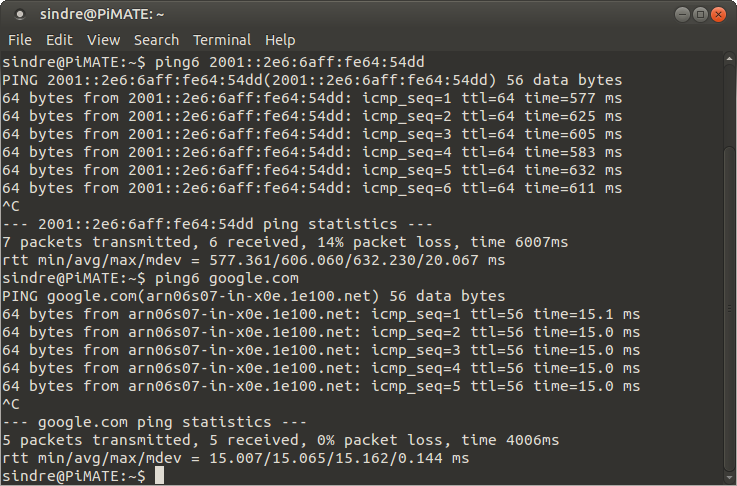
\includegraphics[scale=0.5]{ping6test.png}    
    \caption{Comparison: ping nRF52 and ping google.com}
    \label{fig:pingComparison}
\end{figure}

When tested, the connection turns out to be very slow and in some cases very unstable, especially at maximum transfer rate. In the test of ping shown in figure \ref{fig:pingComparison} the connection between the Raspberry Pi and the nRF52 had 14 \% packet loss, 1 out of 7 packets. Other test showed similar results, but the \gls{coap} \gls{con} has in general got a  higher stability at maximum sending rate than \gls{coap} \gls{non}. After a test period it was therefore decided that the best solution for \gls{non} would be to gather data from sensors at a higher rate, and store them in the nRF52 temporarily. Every second all the measured values are being transferred to the Raspberry Pi, the temporarily values are deleted and the measurement continues. This has proven to be a very stable solution, with successful tests over several days. \gls{con} can handle more frequent transportations than this in this system, on average 4 times per second. See the test shown in chapter \ref{chp:measurements2}.6. \todo{Make figure}. 

\begin{equation} \label{avg_eq}
    \overline{x}_{n} = \frac{\sum\limits_{i=1}^n x_{i}}{n}
\end{equation}

Equation \ref{avg_eq} shows the standard way used to calculate an average of the measured values. Here \textit{a} is any real number and \textit{n} is any integer. 

After a test period, the problems explained in \todo {Skriv om problemer med bt8 i Architecture?} was fixed. A more reliable test could then be performed, as shown in figure \ref{fig:ping2}. Using equation \ref{avg_eq} to calculate average gives an approximate average of 250 ms \gls{rtt}. This is very slow, and way beneath the transfer limitations of both \gls{ble}, \gls{6lowpan} and \gls{coap}, as explained in chapter \ref{chp:background} \todo{Skriv spesifikt om begrensninger for disse tre i background}. Another factor could be limited power supply and computational power, but it is not clear what is the main cause at this point. This will regardless be a huge limitation in the network. 

\begin{figure}[ht]
    \centering
    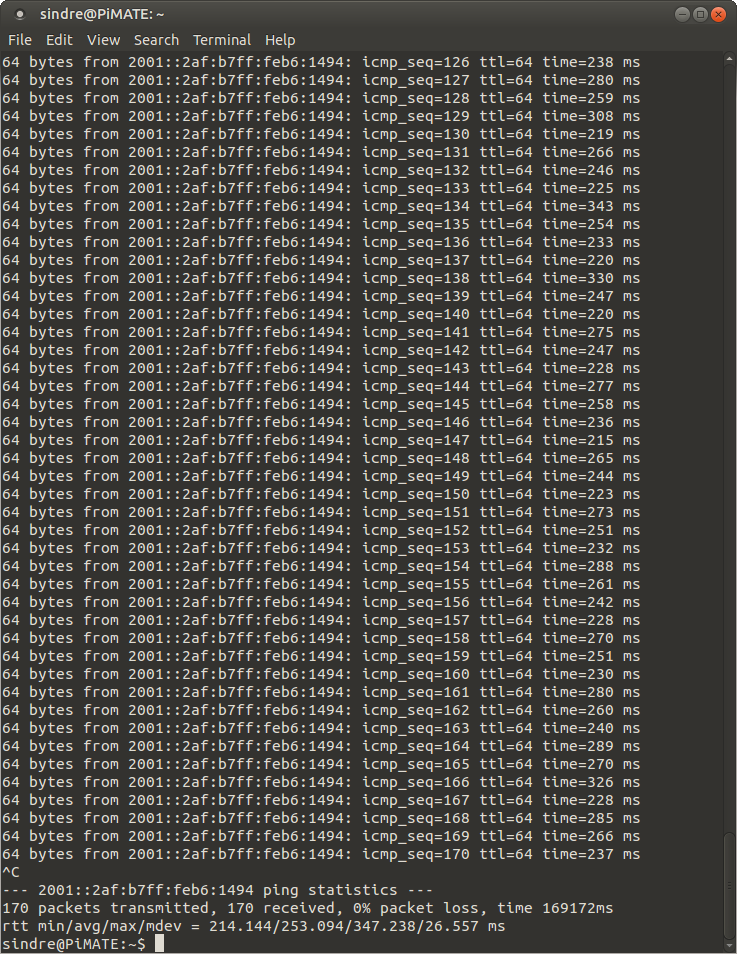
\includegraphics[scale=0.4]{ping3.png}    
    \caption{Ping nRF52, different time}
    \label{fig:ping2}
\end{figure}


The conclusion from these initial tests is therefore that \gls{coap} \gls{con} is stable at at lower transfer interval than \gls{coap} \gls{non}, and can in best case cope with sending every 250th ms, which is very good compared to the high \gls{rtt}. \gls{non} has been so unstable at initial tests that it was decided to only send every second. This makes quite a huge difference when testing the different protocols, as \textit{CoAP CON} can send a lot more \textit{goodput} per second, but \textit{CoAP NON} requires less power to send each message, and a much higher percentage of the packets sent through the network contains useful data.


\subsection{Packet fragmentation}

In Internet Routing, \textit{fragmentation} is known as the action of splitting data into smaller packets, to satisfy the maximal limits of the different technologies or protocols used (e.g. \gls{ble} and \gls{6lowpan} in the network described in this thesis). Each of these packets needs header fields of a certain size, or other requirements. In a network of microcontrollers used in this thesis fragmentation can be a factor that needs to be taken into account to optimize the goodput of the system. This will be a central part of the testing, and will therefore be explained in detail in the following section. 

To better understand fragmentation, imagine a train with carriages as shown in Figure \ref{fig:trainExample}. To be able to operate at all, the train needs a locomotive with an engine driver, a conductor and a cafe carriage. As soon as these things are already there, the company owning the train gets better and better off for every passenger buying a ticket. Lets assume that every carriage can carry 4 employees and 27 passengers, to make it directly comparable to the \gls{ble} packets in the network. Eventually all the carriages will be full, and a decision has to be made if it will be profitable to fit another carriage. It will in general be most profitable to use as many carriages as the locomotive can handle, and to fill up every carriage as much as possible. It will however not be a good idea to connect another carriage if there will only be one additional passenger sitting there, since the extra weight of the carriage adds unnecessary additional weight to the train set compared to the income. 

\begin{figure}[ht]
    \centering
    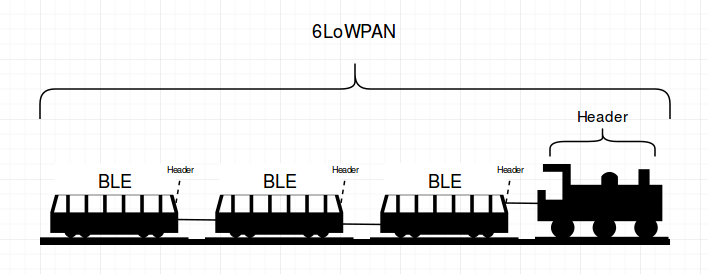
\includegraphics[scale=0.5]{trainExample.png}    
    \caption{Packet fragmentation - train comparison}
    \label{fig:trainExample}
\end{figure}

In this example, the locomotive and employees are the \gls{6lowpan} packet, that are needed no matter what to get the train working. Each additional carriage is a \gls{ble} packet. The goal is therefore to find the maximal number of passengers compared to the cost of adding additional carriages, in other words the maximal number of bytes compared to the number of packets sent. This is known as \textit{fragmentation}, fragmenting data into smaller pieces to satisfy the maximal limitations of packet sizes in the different protocols. This can be exploited by a system developer to maximize \textit{goodput} vs \textit{throughput} in the network.
 


\section{Description of measurements}

The following sections will show experiments performed to to test if \textit{fragmentation} is a huge issiue when sending data through low energy networks, and which of the protocols described in chapter \ref{chp:background}  is the most efficient to use when the goal is to get as high \textit{googput} as possible. This will be done by sending data of constant length, capture packets using \textit{Wireshark}, and then increasing the packet size to see the changes. 

Before these experiements started, the expected results was that sending a small amount of data at a time would not be preferable, because of the needed bytes to set up the connection, header files and so on. It was not known how big the packages needed to be before it would be considered \textit{profitable} to send. 

When sending \gls{ble} packets over the network, observations from the system shows that the maximum packet size over \gls{ble} is 31 bytes. Each of these packages needs a header field of 4 bytes, meaning 27 bytes left for useful data. However, to start the connection at all, 76 byte is needed, meaning three \gls{ble} packets. The ratio between \textit{useful} and \textit{needed} (known as \textit{goodput} and \textit{throughput}) data transferred therefore start out very poorly if the payload sent is very small.The best possible percentage of useful data we can hope to acheive will also be limited by this, 27 bytes goodput and 4 bytes header field, shown in the following calculation.  

\begin{equation} \label{percentage_eq} 
	\delta = \frac{x_{2}}{x_{1}} * 100 \%
\end{equation}

Equation \ref{percentage_eq} shows the standard way used to calculate the percentage, \textdelta , that the natural number \textit{x\textsubscript{2}} is of the total amount \textit{x\textsubscript{1}}. 

\begin{equation}
    \frac{27 b}{31 b}*100 \% = 87,094776 \% \approx 87,1 \%
\end{equation}





In the actual system the number will quite certain be a lot lower than this. Both because header files in \gls{6lowpan} packages needs to use some of the capacity, and because of other limitations\todo{Like what?}. 


\section{CoAP}

As explained in Chapter \ref{chp:measurements2}.1.1, \gls{coap} can be split into two different main sections. \gls{con} messages can be sent quite frequently, but every message needs to get an \gls{ack} before the next message can be sent. This means that it is quite fast, but a lot of packets needs to be transported through to get usable data at the other end. The other alternative is \gls{non}, where each message does \textit{not} need an \gls{ack}. 


%\begin{figure}[ht]
%    \centering
%    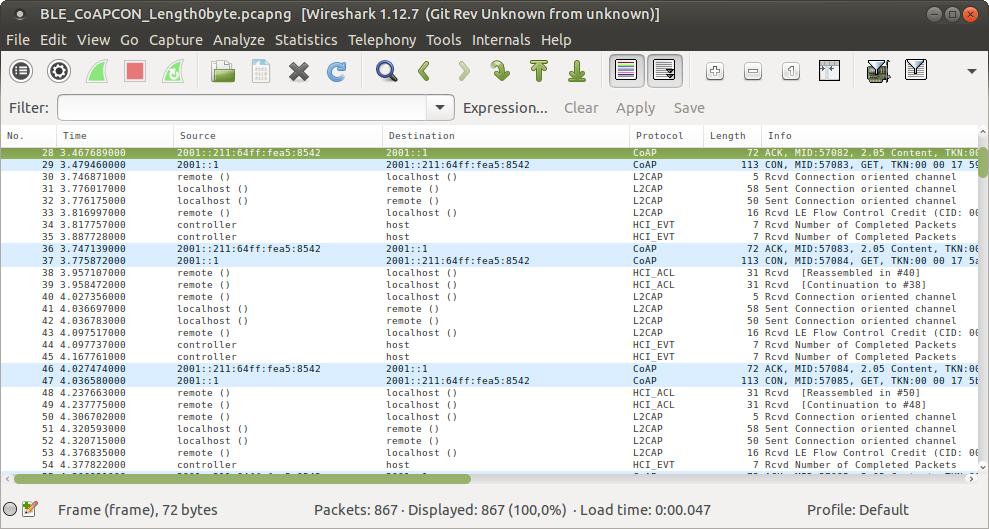
\includegraphics[width=\textwidth]{wiresharkCoAPCON0byte.png}    
%    \caption{Wireshark capture, CoAP CON, 0 bytes goodput}
%    \label{fig:coapCON0Wireshark}
%\end{figure}



%\begin{figure}[ht]
%    \centering
%    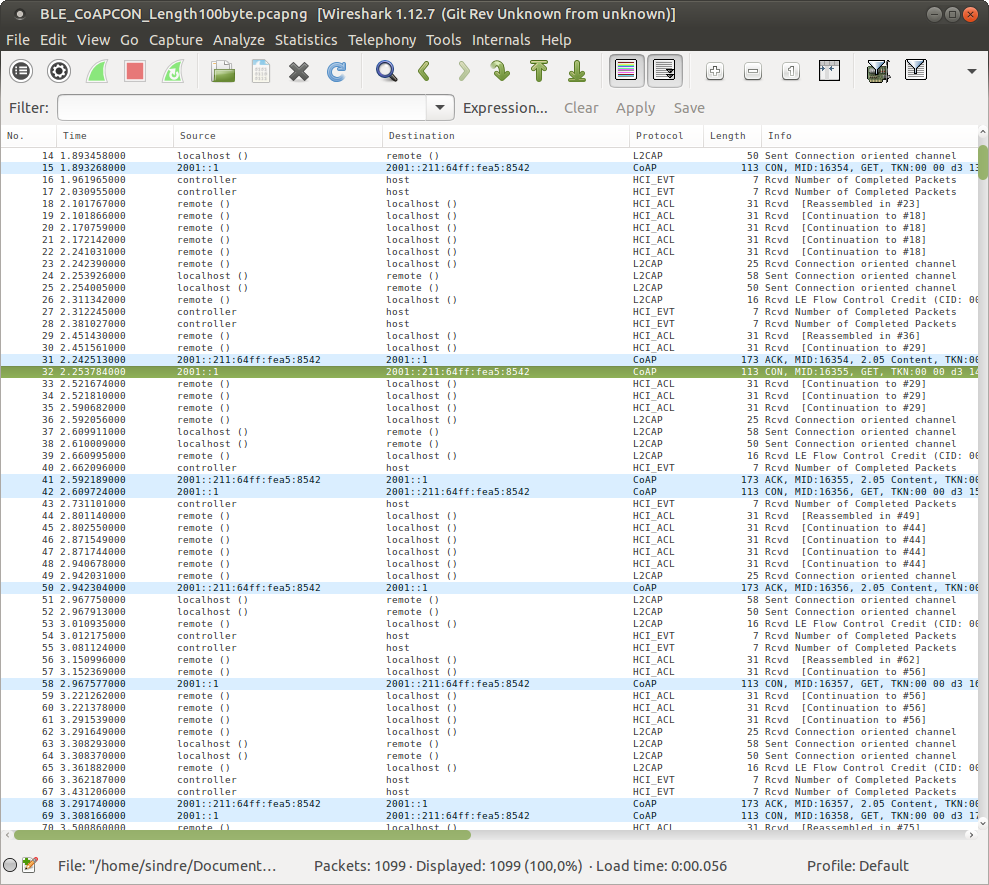
\includegraphics[width=\textwidth]{wiresharkCON100bytes.png}    
%    \caption{Wireshark capture, CoAP CON, 100 bytes goodput}
%    \label{fig:coapCON100Wireshark}
%\end{figure}

\begin{table}[ht]
\centering
\caption{Wireshark CoAP CON 0 bytes}
\label{coapCON0table}
\begin{tabular}{lllll}
Number & Time   & Protocol & Length & Info                             \\ \hline
36     & 3.7471 & CoAP     & 72     & ACK, MID:57083, 2.05 Content     \\
37     & 3.7759 & CoAP     & 113    & CON, MID:57084, GET              \\
38     & 3.9571 & HCI\_ACL & 31     & Rcvd {[}Reassembled in \#40{]}   \\
39     & 3.9584 & HCI\_ACL & 31     & Rcvd {[}Continuation to \#38{]}  \\
40     & 4.0274 & L2CAP    & 5      & Rcvd Connection oriented channel \\
41     & 4.0367 & L2CAP    & 58     & Sent Connection oriented channel \\
42     & 4.0368 & L2CAP    & 50     & Sent Connection oriented channel \\
43     & 4.0975 & L2CAP    & 16     & Rcvd LE Flow Control             \\
44     & 4.0977 & HCI\_EVT & 7      & Rcvd Number of Completed Packets \\
45     & 4.1678 & HCI\_EVT & 7      & Rcvd Number of Completed Packets \\
46     & 4.0275 & CoAP     & 72     & ACK, MID:57084, 2.05 Content     \\
47     & 4.0366 & CoAP     & 113    & CON, MID:57085, GET              \\ \hline
\end{tabular}
\end{table}

Table \ref{coapCON0table} shows the most basic example of a capture of packets in Wireshark. The full capture can be seen in the Appendix \ref{chp:appendix}. In this case an empty char array was sent, meaning an goodput equal to 0 byte. All of these bytes are therefore sent to route packages through the network. The maximum of 31 bytes per \gls{ble} packet have been exceeded twice, meaning that three packets needed to be sent. The first packet is labeled \textit{[Reassembled in \#40]}, the second \textit{[Continuation to \#38]} and the last \textit{Connection oriented channel}. After this, the \gls{ack} packages follows, two packages of 58 and 50 bytes, respectively. The last bytes received tells how many packages was completed, as a built in feature in \gls{ble}  \gls{hci}  and \gls{acl}. All of these packages can fit into one \gls{6lowpan} packet, since the total number of bytes are less than 270 bytes. 

Note that packet number 46 and 47 in table \ref{coapCON0table} has got a timestamp that indicates that they originally was sent from the end node in the network as packet number 41 and 42, but used longer time than the other packets sent through the network at the same time. The main reason for this is of course that they are bigger than the rest of the packets, but since the network limit should be much higher than this it can maybe be seen as a weakness that this gives a clear impact even at these small values.  


\begin{table}[]
\centering
\caption{Wireshark CoAP CON 100 bytes}
\label{coapCON100table}
\begin{tabular}{lllll}
Number & Time   & Protocol & Length & Info                             \\ \hline
29     & 2.4514 & HCI\_ACL & 31     & Rcvd {[}Reassembled in \#36{]}   \\
30     & 2.4516 & HCI\_ACL & 31     & Rcvd {[}Continuation to \#29{]}  \\
31     & 2.2425 & CoAP     & 173    & ACK, MID:16354, 2.05 Content     \\
32     & 2.2538 & CoAP     & 113    & CON, MID:16355, GET              \\
33     & 2.5217 & HCI\_ACL & 31     & Rcvd {[}Continuation to \#29{]}  \\
34     & 2.5218 & HCI\_ACL & 31     & Rcvd {[}Continuation to \#29{]}  \\
35     & 2.5907 & HCI\_ACL & 31     & Rcvd {[}Continuation to \#29{]}  \\
36     & 2.5921 & L2CAP    & 25     & Rcvd Connection oriented channel \\
37     & 2.6099 & L2CAP    & 58     & Sent Connection oriented channel \\
38     & 2.6100 & L2CAP    & 50     & Sent Connection oriented channel \\
39     & 2.6610 & L2CAP    & 16     & Rcvd LE Flow Control             \\
40     & 2.6621 & HCI\_EVT & 7      & Rcvd Number of Completed Packets \\
41     & 2.5922 & CoAP     & 173    & ACK, MID:16355, 2.05 Content     \\
42     & 2.3097 & CoAP     & 113    & CON, MID:16356, GET              \\ 
43     & 2.7311 & HCI\_EVT & 7      & Rcvd Number of Completed Packets \\ \hline
\end{tabular}
\end{table}

In table \ref{coapCON100table}, 100 bytes of goodput is being sent through. The same basic packages needed are still there, but in addition the 100 bytes of data is added. This means adding more \gls{ble} packets, but also that the percentage of useful data sent through is a lot higher, approximatley 55 \% in this case. By doing several experiments like this, it was possible to create the graph in Figure \ref{fig:coapCON0200}. This shows the correlation between goodput and throughput compared to the number of packets sent, measured every 10th byte from 0 byte to 200 bytes large packets.


\begin{figure}[ht]
    \centering
    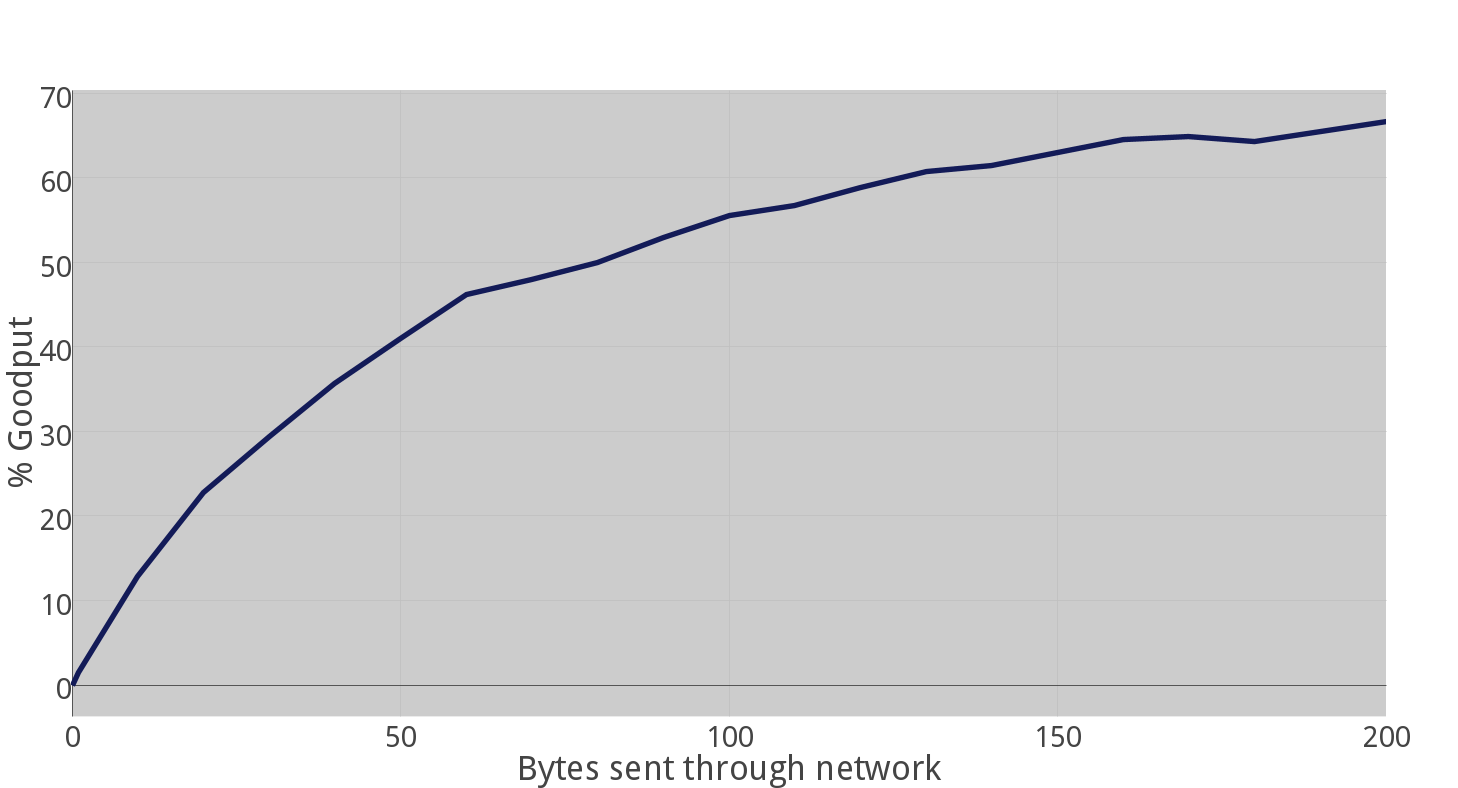
\includegraphics[scale=1.0]{CON0to200plot09thickerGRAY.png}    
    \caption{CoAP CON, 0-200 bytes sent}
    \label{fig:coapCON0200}
\end{figure}



In this particular case shown in \ref{fig:coapCON0200} it makes no sense to send less than 50 bytes of useful data at once, since more than 50 \% of the bytes sent will be header files. This is comparable to having a locomotive and full crew at disposal, but only a few or none paying passengers. The best possible result is to have every carriage full, with 27 passengers and 4 employees. Since at least 4 bytes out of every 31 sent needs to be used to header information, the best possible result will be 87,1 \%, as shown in equation 4.1. In mathematics, this is described as a \textit{horizontal asymptote} since the distance between the graph and \textit{y = 87,1} will approach zero after an infinite number of bytes has been transferred. The graph will therefore converge to 87,1 \%, just as the values climbing in figure \ref{fig:coapCON0200}, even before packet size of 200 bytes.  

\subsection{Discussion}

Even though this first test was done with a very limited amount of data transferred, it is easy to see that the curve clearly flattens out and forms the shape of a \textit{\gls{parabola}} with a vertical \textit{\gls{directrix}} at \textit{x = 0}. The next step would be to transfer a larger amount of data, to verify that the assumptions that the graph will converge to the asymptotic value \textit{y = 87,1} when $lim_{x\to\infty}$. The limitations of transfer rate is not nearly yet met by either \gls{ble} or \gls{6lowpan}. This test will therefore be explained in the next section. 


Since there is already a clear trend in the form of the graph in figure \ref{fig:coapCON0200} even before the transfer rate reaches 200 bytes, it makes sense to also test the other version included in \gls{coap}, \gls{con}. If it is possible to find a way of transportation that could give a higher mathematical maximum, and also get to this limit faster, it could be very profitable to the system. It also makes sense to test \gls{coap} \gls{non} because it doesn’t need to send an \gls{ack} for every packet, as \gls{con} does. Maybe this means that the header files can be split up in another way, and that the useful amount of data sent through therefore will be higher. 


%\subsection{CoAP CON with more data}

To see what happened when the limit of a \gls{6lowpan} packet was breached in the system, tests was being set up to send larger amounts of data than 200 bytes. This would also be a good way to test if the percentage of goodput will converge to 87,1 \%, only considering \gls{ble} packets. The following test and examples will therefore send a fixed number of bytes at once from 0 to 1000 bytes (1 kB), with a 50 byte interval. As before, the messages are being sent as soon as possible, meaning approximately four messages per second on average using \gls{coap} \gls{con}. In addition will \gls{non} be tested in detail. 

%\begin{figure}[ht]
%    \centering
%    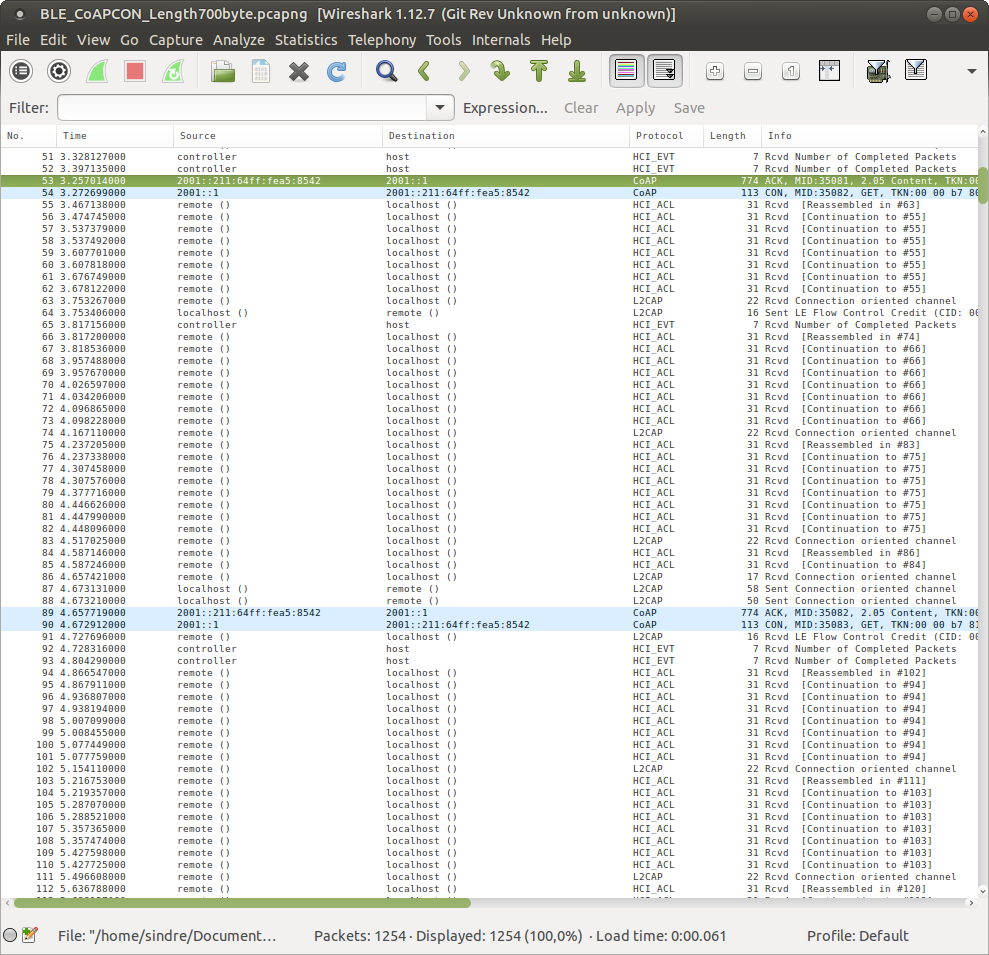
\includegraphics[width=\textwidth]{Wireshark700bytes2.png}    
%    \caption{Wireshark capture, CoAP CON, 700 bytes goodput}
%   \label{fig:coapCON700Wireshark}
%\end{figure}

\subsection{CoAP NON comparison}

A \gls{coap} \gls{non} request does not require a response in form of an \gls{ack}. This means that the 108 bytes sent to and handled by the end node can be skipped, which means less computational power in the end node and network capacity to the node is needed. This solution makes sense to use in networks where the demand for all data is low, since packets can be lost without the use of \glspl{ack}. As explained in chapter \ref{chp:measurements2}.1.1, the transfer frequency is limited using \gls{non} in this system, due to unstable results in tests at the beginning of the set up. The transfer rate is therefore set to one per second for this protocol. 

\todo{4 LEDs image?}

\begin{table}[ht]
\centering
\caption{Wireshark CoAP NON 0 bytes}
\label{coapNON0table}
\begin{tabular}{lllll}
\hline
Number & Time    & Protocol & Length & Info                             \\ \hline
%\rowcolor{blue} 
90     & 23.0405 & HCI\_ACL & 31     & Rcvd {[}Reassembled in \#92{]}   \\
91     & 23.0411 & HCI\_ACL & 31     & Rcvd {[}Continuation to \#90{]}  \\
92     & 23.1107 & L2CAP    & 9      & Rcvd Connection oriented channel \\
93     & 23.1109 & CoAP     & 76     & NON, MID:14, 2.05 Content        \\ \hline
\end{tabular}
\end{table}


A basic example of the \gls{coap} \gls{non} connection is shown in table \ref{coapNON0table}. The entire Wireshark capture can be seen in Appendix \ref{chp:appendix}. This is directly comparable to table \ref{coapCON0table}, that shows a Wireshark capture of \gls{coap} \gls{con} packages. It is easy to see that a lot fewer packages needs to be sent using \gls{ble}, without the use of \glspl{ack}. The total amount of bytes sent is 31+31+9=71 bytes, meaning three \gls{ble} packages and one \gls{6lowpan} packet. This is less than half of what was needed using \gls{coap} \gls{con}, where the 108 \gls{ack} packages was needed in addition. The packets are still recognizable the same way as before, the first packet is labeled \textit{[Reassembled in \#40]}, the second \textit{[Continuation to \#38]} and the last \textit{Connection oriented channel}.

Fewer packages sent means less energy used, less network capacity needed and less computational power in the end node. Hopefully this will lead to a higher percentage of goodput compared to throughput as well. it would therefore be interesting to compare the rest of the measured values.

\begin{table}[]
\centering
\caption{Wireshark CoAP NON 100 bytes}
\label{coapNON100table}
\begin{tabular}{lllll}
\hline
Number & Time    & Protocol & Length & Info   							  \\ \hline                          
39     & 11.0363 & CoAP     & 177    & NON, MID:2, 2.05 Content         \\
40     & 11.9452 & HCI\_ACL & 31     & Rcvd {[}Reassembled in \#45{]}   \\
41     & 11.9465 & HCI\_ACL & 31     & Rcvd {[}Continuation to \#40{]}  \\
42     & 12.0154 & HCI\_ACL & 31     & Rcvd {[}Continuation to \#40{]}  \\
43     & 12.0168 & HCI\_ACL & 31     & Rcvd {[}Continuation to \#40{]}  \\
44     & 12.0857 & HCI\_ACL & 31     & Rcvd {[}Continuation to \#40{]}  \\
45     & 12.0858 & L2CAP    & 29     & Rcvd Connection oriented channel \\
46     & 12.0860 & CoAP     & 177    & NON, MID:3, 2.05 Content         \\ \hline
\end{tabular}
\end{table}

Table \ref{coapNON100table} shows the case where 100 bytes of data are sent using \gls{coap} \gls{non}. This is directly comparable to the test shown in table \ref{coapCON100table}, where the same amount of data is sent over \gls{con}. The overall structure is the same as before. Since it is only one packet noted \textit{Reassembled in \#n}, which marks the beginning of a new \gls{6lowpan} packet. The total amount sent must therefore be under 270 bytes, which makes sense. The \gls{non} packet size is here 177 bytes, compared to 173 bytes in \gls{con}, which represents one more header field of 4 bytes needed in \gls{non}. Overall a small difference in the packets containing data, but as expected a lot more packets needs to be sent in total in \gls{con}.


Using these measurements the following plot could be drawn. 

%\begin{figure}[ht]
%    \centering
%    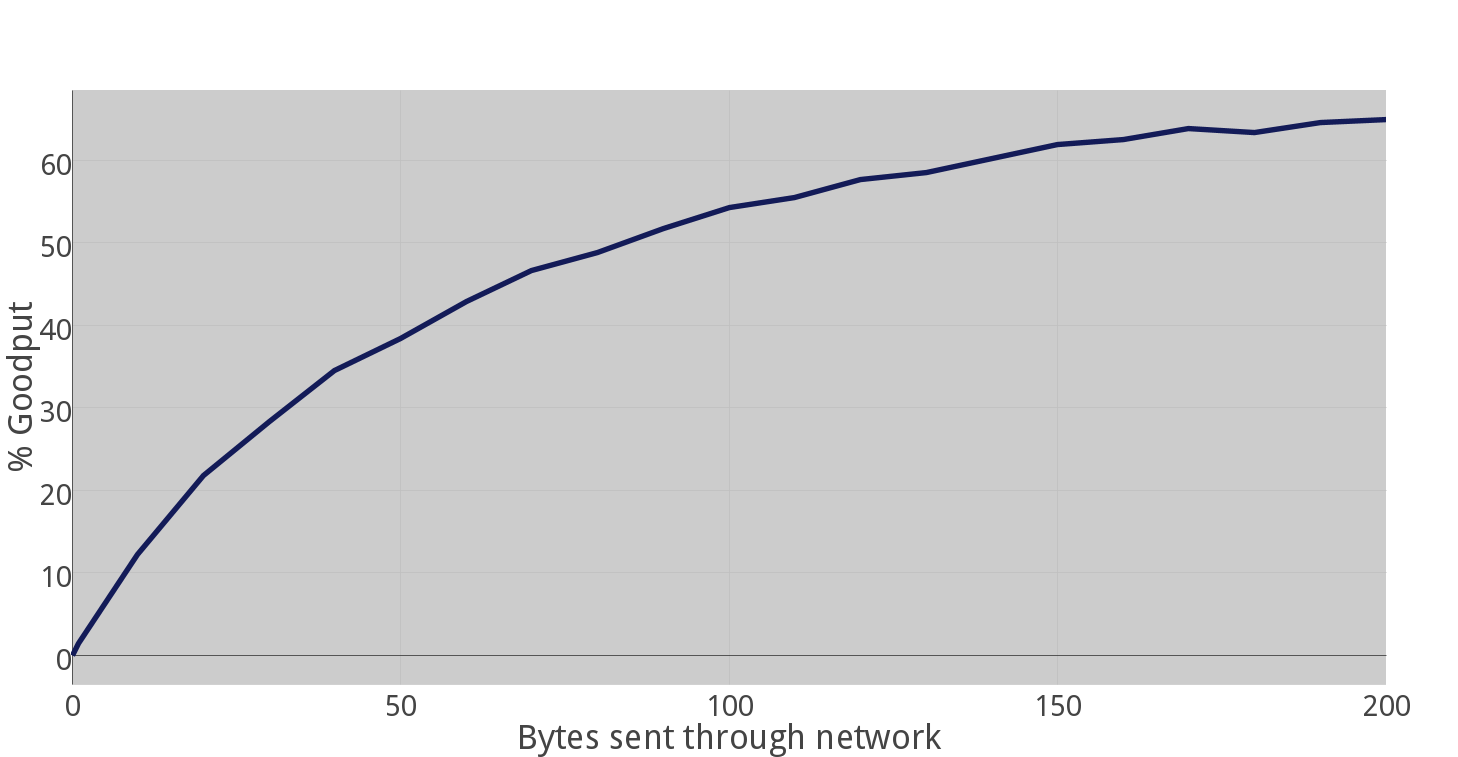
\includegraphics[scale=1.0]{NON0to200plotx09_thickerLineGRAY.png}    
%    \caption{NON 0-200 bytes }
%    \label{fig:NON0-200b}
%\end{figure}




\begin{figure}[ht]
    \centering
    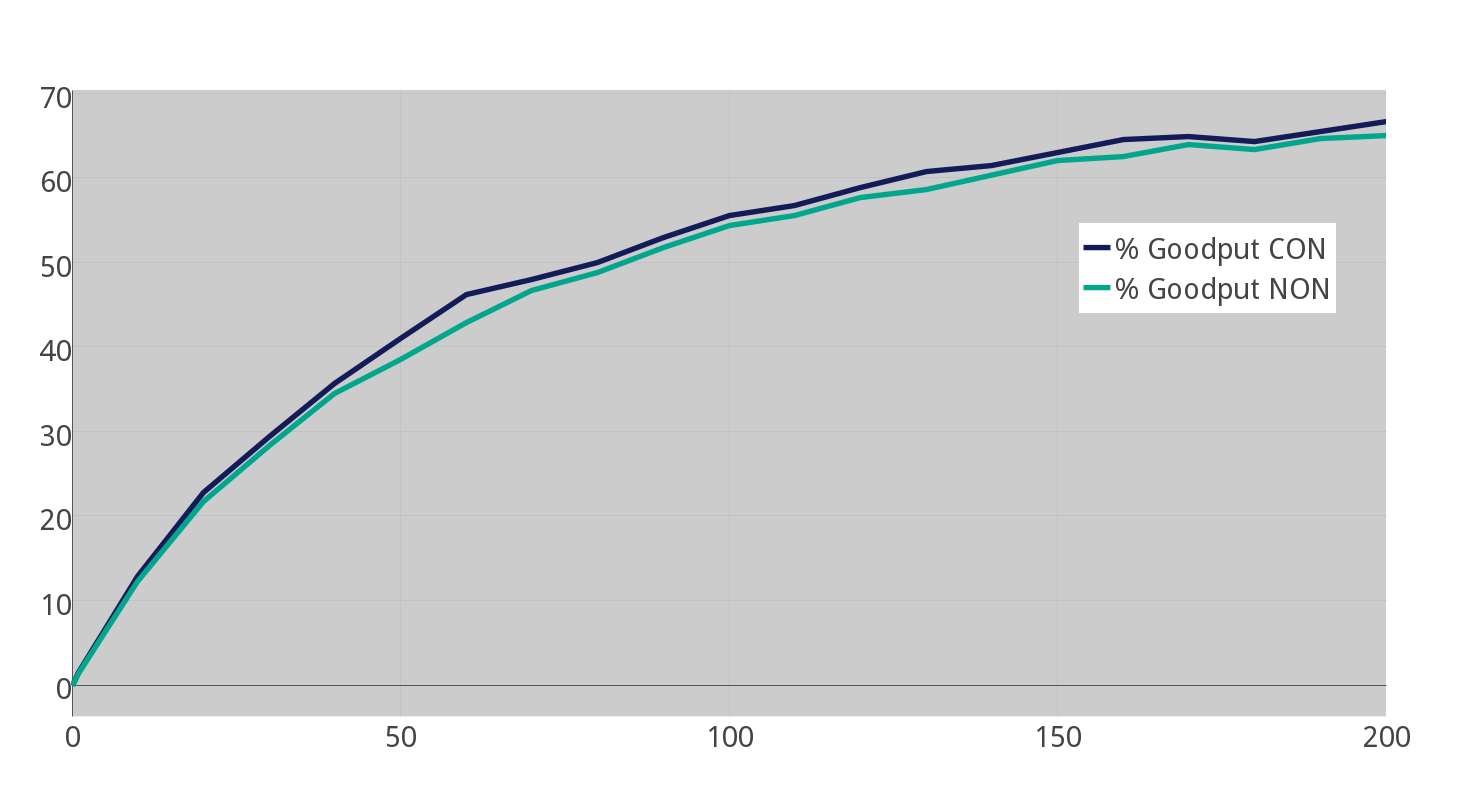
\includegraphics[scale=1.0]{CONvsNONplot_0-200_thickerGRAY.png}    
    \caption{CON vs NON 0-200 bytes}
    \label{fig:CONvsNON0-200}
\end{figure}

Figure \ref{fig:CONvsNON0-200} shows the comparison between sending between 0 and 200 bytes of useful data through the network at once. Keep in mind that this does not show sending rate per time (which will be discussed in chapter \todo{write chapter}), but percentage of the data sent that is useful data. \gls{con} can be sent much more often than \gls{non} in practice. It could therefore maybe be expected that this could give \gls{non} an advantage. \todo{<- Re-write}. \gls{non} does not need to send \glspl{ack} for every package, which should be an advantage concerning to maximize throughput. Still it is the more complex and more frequently sent \gls{con} that gets the best results in this test, with a small margin. 


\subsection{CoAP, testing with more data}

Table \ref{coapCON700table} shows a bigger and more complex case, where 700 bytes of data are being sent at once. In total 889 bytes are being sent, with a \gls{con} packet size of 774 bytes. This gives a percentage of goodput at 78.74 \%. The maximum packet length of a \gls{6lowpan} packet in this system of 270 bytes is therefore exceeded, as we can see in the figure. After 8 \gls{ble} packages of 31 bytes each has been sent, there is only room for 22 bytes in the last packet before the \gls{6lowpan} packet is full. This is repeated several times, once for each \gls{6lowpan} packet, until the last \gls{ble} packets at the size of 17 bytes. After this the standard packages for \gls{ack} and \textit{Number of completed packages} follows. This is in general a good example on how fragmentation of packets works in this system. 

\begin{table}[h]
\centering
\caption{Wireshark CoAP CON 700 bytes}
\label{coapCON700table}
\begin{tabular}{lllll}
\hline
Number & Time    & Protocol & Length & Info                             \\ \hline
%\rowcolor{blue} 
53     & 3.2570  & CoAP     & 774    & ACK, MID:35081, 2.05 Content     \\
%\rowcolor{38FFF8} 
54     & 3.2727  & CoAP     & 113    & CON, MID:35082, GET	              \\
55     & 3.4671  & HCI\_ACL & 31     & Rcvd {[}Reassembled in \#63{]}   \\
56     & 3.4747  & HCI\_ACL & 31     & Rcvd {[}Continuation to \#55{]}  \\
57     & 3.5374  & HCI\_ACL & 31     & Rcvd {[}Continuation to \#55{]}  \\
58     & 3.5375  & HCI\_ACL & 31     & Rcvd {[}Continuation to \#55{]}  \\
59     & 3.6077  & HCI\_ACL & 31     & Rcvd {[}Continuation to \#55{]}  \\
60     & 3.6078  & HCI\_ACL & 31     & Rcvd {[}Continuation to \#55{]}  \\
61     & 3.6767  & HCI\_ACL & 31     & Rcvd {[}Continuation to \#55{]}  \\
62     & 3.6782  & HCI\_ACL & 31     & Rcvd {[}Continuation to \#55{]}  \\
63     & 3.7533  & L2CAP    & 22     & Rcvd Connection oriented channel \\
64     & 3.7534  & L2CAP    & 16     & Sent LE Flow Control             \\
65     & 3.8172  & HCI\_EVT & 7      & Rcvd Number of Completed Packets \\
66     & 3.8172  & HCI\_ACL & 31     & Rcvd {[}Reassembled in \#74{]}   \\
67     & 3.8185  & HCI\_ACL & 31     & Rcvd {[}Continuation to \#66{]}  \\
68     & 3.9575  & HCI\_ACL & 31     & Rcvd {[}Continuation to \#66{]}  \\
69     & 3.9577  & HCI\_ACL & 31     & Rcvd {[}Continuation to \#66{]}  \\
70     & 4.0266  & HCI\_ACL & 31     & Rcvd {[}Continuation to \#66{]}  \\
71     & 4.0342  & HCI\_ACL & 31     & Rcvd {[}Continuation to \#66{]}  \\
72     & 4.0979  & HCI\_ACL & 31     & Rcvd {[}Continuation to \#66{]}  \\
73     & 4.0982  & HCI\_ACL & 31     & Rcvd {[}Continuation to \#66{]}  \\
74     & 4.1671  & L2CAP    & 22     & Rcvd Connection oriented channel \\
75     & 4.2372  & HCI\_ACL & 31     & Rcvd {[}Reassembled in \#83{]}   \\
76     & 4.2373  & HCI\_ACL & 31     & Rcvd {[}Continuation to \#75{]}  \\
77     & 4.3075  & HCI\_ACL & 31     & Rcvd {[}Continuation to \#75{]}  \\
78     & 4.3076  & HCI\_ACL & 31     & Rcvd {[}Continuation to \#75{]}  \\
79     & 4.3777  & HCI\_ACL & 31     & Rcvd {[}Continuation to \#75{]}  \\
80     & 4.4466  & HCI\_ACL & 31     & Rcvd {[}Continuation to \#75{]}  \\
81     & 4.4480  & HCI\_ACL & 31     & Rcvd {[}Continuation to \#75{]}  \\
82     & 4.4481  & HCI\_ACL & 31     & Rcvd {[}Continuation to \#75{]}  \\
83     & 4.5170  & L2CAP    & 22     & Rcvd Connection oriented channel \\
84     & 4.5871  & HCI\_ACK & 31     & Rcvd {[}Reassembled in \#86{]}   \\
85     & 4.5875  & HCI\_ACL & 31     & Rcvd {[}Continuation to \#84{]}  \\
86     & 4.6574  & L2CAP    & 17     & Rcvd Connection oriented channel \\
87     & 4.6731  & L2CAP    & 58     & Rcvd Connection oriented channel \\
88     & 4.6732  & L2CAP    & 50     & Rcvd Connection oriented channel \\
%\rowcolor[HTML]{38FFF8} 
89     & 4.6577  & CoAP     & 774    & ACK, MID:35082, 2.05 Content     \\
%\rowcolor[HTML]{38FFF8} 
90     & 4.6729  & CoAP     & 113    & NON, MID:35083, GET              \\ \hline
\end{tabular}
\end{table}


\newpage

\begin{figure}[ht]
    \centering
    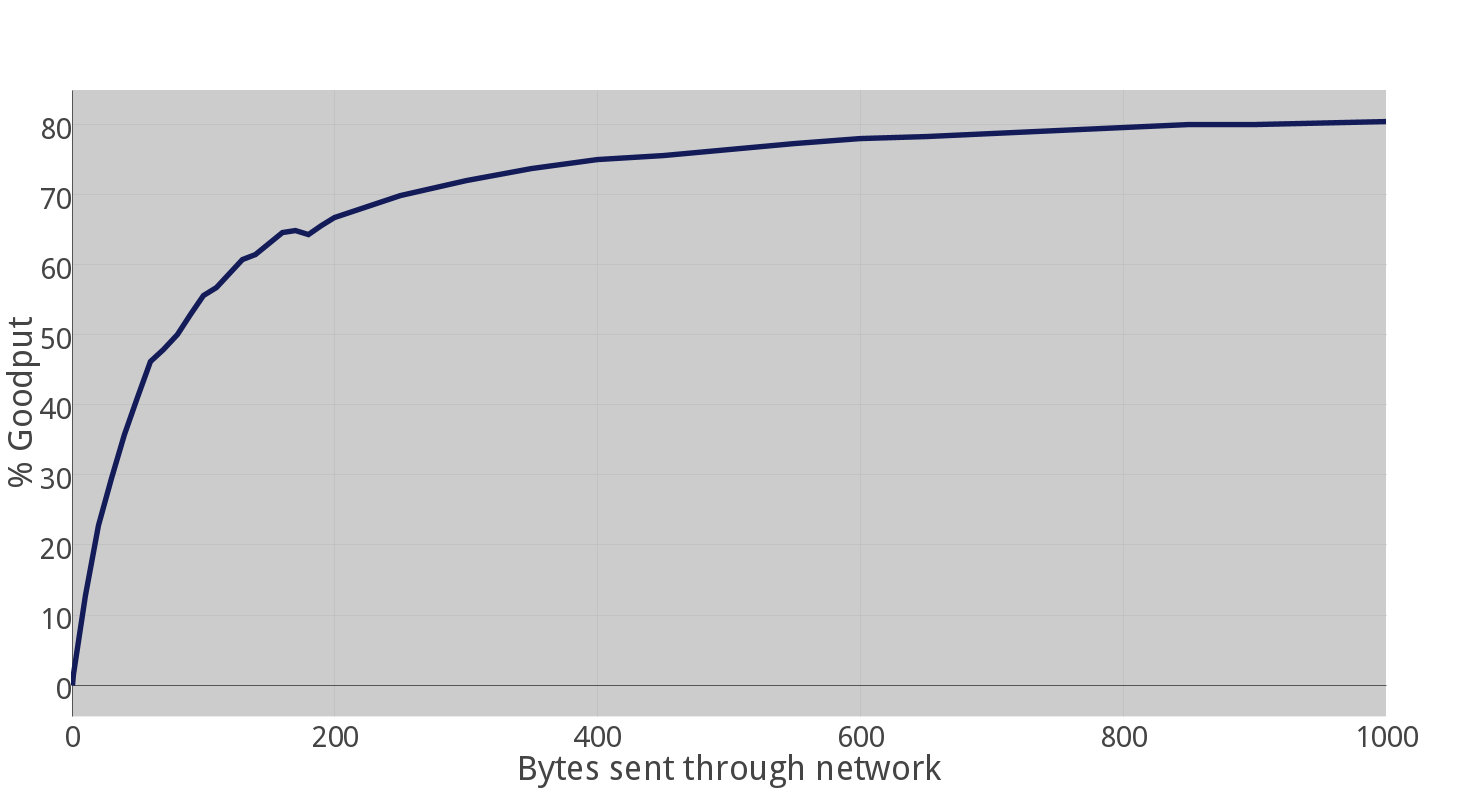
\includegraphics[width=\textwidth]{CON0toK_thickerGRAY.png}    
    \caption{CoAP CON plot, 200 bytes to 1 kB}
    \label{fig:plotCoAPCON200toK}
\end{figure}

Using these results it was possible to plot the graph in figure \ref{fig:plotCoAPCON200toK} \todo{Make graph more clear}. Here it is easy to see the same trends as in  \ref{fig:coapCON0200}, but in more detail over a wider span of bytes sent. These results are as expected after the previous tests, and in compliance with the calculations done in equation 4.1. 

In this example points in the graph was denoted every 50th byte sent. This gives us \todo{set in graph for 0-1000 before this, to see the flatness?}


%\begin{figure}[ht]
%    \centering
%    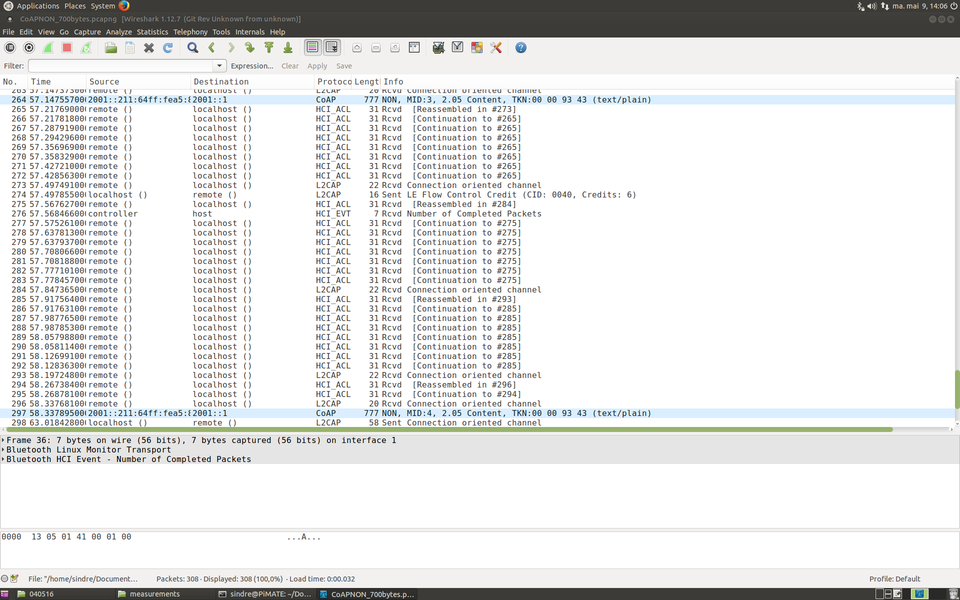
\includegraphics[scale=0.40]{rsz_1coapnon_wireshark700fullscreen.png}    
%    \caption{CoAP NON 700 bytes Wireshark capture}
%    \label{fig:NON7000bytesFullWireshark}
%\end{figure}

 


\begin{table}[ht]
\centering
\caption{Wireshark CoAP NON 700 bytes}
\label{coapNON700table}
\begin{tabular}{lllll}
\hline
Number & Time    & Protocol & Length & Info                             \\ \hline
264    & 57.1476 & CoAP     & 777    & NON, MID:3, 2.05 Content         \\
265    & 57.2177 & HCI\_ACL & 31     & Rcvd {[}Reassembled in \#273{]}  \\
266    & 57.2178 & HCI\_ACL & 31     & Rcvd {[}Continuation to \#265{]} \\
267    & 57.2879 & HCI\_ACL & 31     & Rcvd {[}Continuation to \#265{]} \\
268    & 57.2943 & HCI\_ACL & 31     & Rcvd {[}Continuation to \#265{]} \\
269    & 57.3570 & HCI\_ACL & 31     & Rcvd {[}Continuation to \#265{]} \\
270    & 57.3583 & HCI\_ACL & 31     & Rcvd {[}Continuation to \#265{]} \\
271    & 57.4272 & HCI\_ACL & 31     & Rcvd {[}Continuation to \#265{]} \\
272    & 57.4286 & HCI\_ACL & 31     & Rcvd {[}Continuation to \#265{]} \\
273    & 57.4975 & L2CAP    & 22     & Rcvd Connection oriented channel \\
274    & 57.4979 & L2CAP    & 16     & Sent LE Flow Control             \\
275    & 57.5676 & HCI\_ACL & 31     & Rcvd {[}Reassembled in \#284{]}  \\
276    & 57.5685 & HCI\_EVT & 7      & Rcvd Number of Completed Packets \\
277    & 57.5753 & HCI\_ACL & 31     & Rcvd {[}Continuation to \#275{]} \\
278    & 57.6378 & HCI\_ACL & 31     & Rcvd {[}Continuation to \#275{]} \\
279    & 57.6379 & HCI\_ACL & 31     & Rcvd {[}Continuation to \#275{]} \\
279    & 57.7080 & HCI\_ACL & 31     & Rcvd {[}Continuation to \#275{]} \\
280    & 57.7082 & HCI\_ACL & 31     & Rcvd {[}Continuation to \#275{]} \\
281    & 57.7771 & HCI\_ACL & 31     & Rcvd {[}Continuation to \#275{]} \\
282    & 57.7785 & HCI\_ACL & 31     & Rcvd {[}Continuation to \#275{]} \\
283    & 57.7785 & HCI\_ACL & 31     & Rcvd {[}Continuation to \#275{]} \\
284    & 57.8474 & L2CAP    & 22     & Rcvd Connection oriented channel \\
285    & 57.9176 & HCI\_ACL & 31     & Rcvd {[}Reassembled in \#293{]}  \\
286    & 57.9176 & HCI\_ACL & 31     & Rcvd {[}Continuation to \#285{]} \\
287    & 57.9878 & HCI\_ACL & 31     & Rcvd {[}Continuation to \#285{]} \\
288    & 57.9879 & HCI\_ACL & 31     & Rcvd {[}Continuation to \#285{]} \\
289    & 58.0580 & HCI\_ACL & 31     & Rcvd {[}Continuation to \#285{]} \\
290    & 58.0581 & HCI\_ACL & 31     & Rcvd {[}Continuation to \#285{]} \\
291    & 58.1270 & HCI\_ACL & 31     & Rcvd {[}Continuation to \#285{]} \\
292    & 58.1284 & HCI\_ACL & 31     & Rcvd {[}Continuation to \#285{]} \\
293    & 58.1972 & L2CAP    & 22     & Rcvd Connection oriented channel \\
294    & 58.2673 & HCI\_ACK & 31     & Rcvd {[}Reassembled in \#296{]}  \\
295    & 58.2688 & HCI\_ACL & 31     & Rcvd {[}Continuation to \#294{]} \\
296    & 58.3378 & L2CAP    & 20     & Rcvd Connection oriented channel \\
297    & 58.3379 & CoAP     & 777    & NON, MID:4, 2.05 Content         \\ \hline
\end{tabular}
\end{table}

\newpage

Table \ref{coapNON700table} shows the case where 700 bytes where sent at once through the network, using \gls{coap} \gls{non}. The \gls{non} packet size is at 777 bytes, which is as expected from the previous tests. This means 4 bytes larger than the same test using \gls{con}, meaning an additional header field. 

\begin{equation} \label{lessThanHAlfAPercentCalculation}
    \frac{78,47}{78,74} \approx 0,9966  \rightarrow 100 \% - 99,66 \% = 0,34 \%
\end{equation}


Calculations in equation \ref{lessThanHAlfAPercentCalculation} show that the goodput here is 78,47 \%, compared to 78,74 \% in \gls{con}. The difference between these two is \textit{0,34 \%}, which in this case is considered \textit{very} small. This can also be seen clearly in \ref{fig:CONvsNON0-1000}. Because of this, it was concluded that the results for using \gls{non} and \gls{con} can be considered as negligible for transmissions larger than 1 kB. Tests with larger amounts of data than this at once was therefore not conducted in this project.  



\begin{figure}[ht]
    \centering
    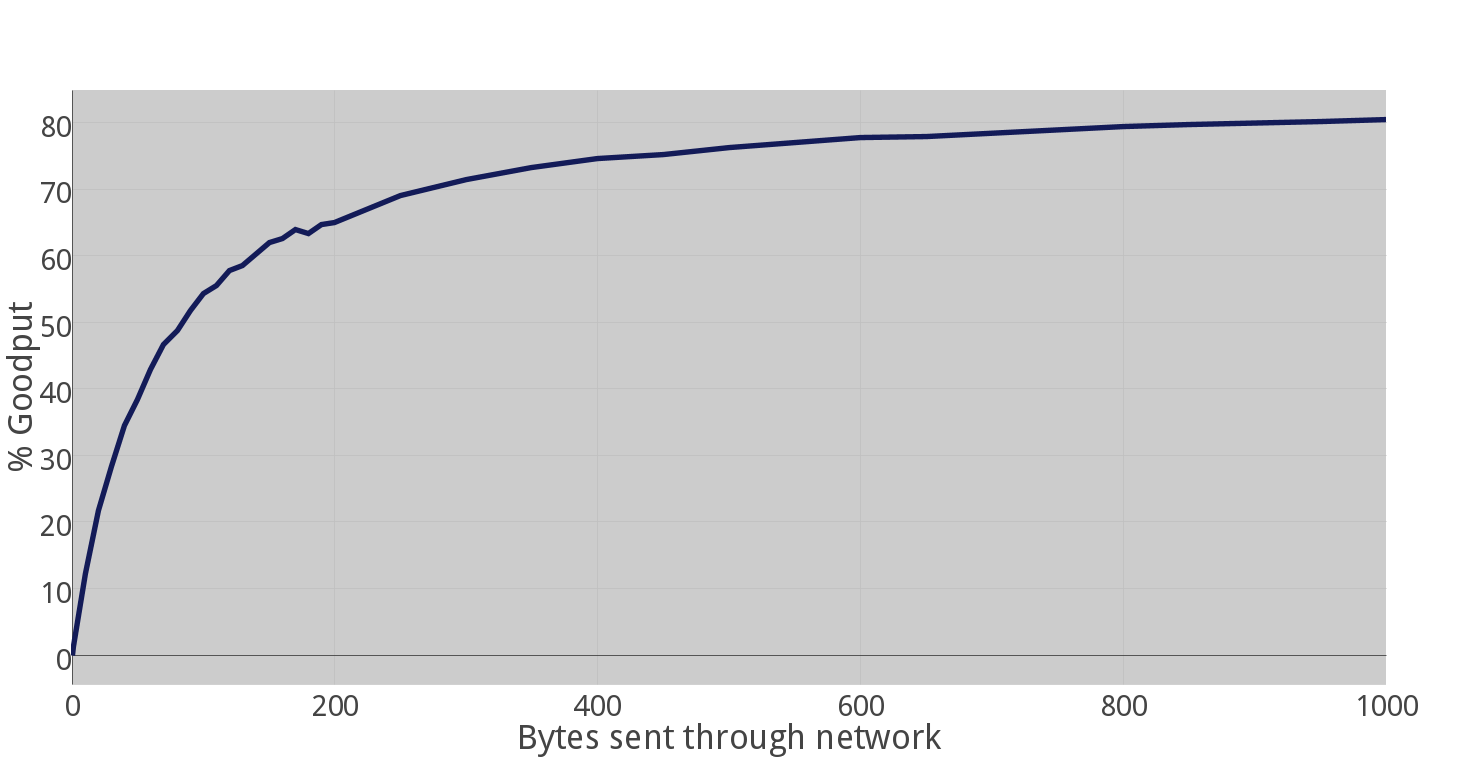
\includegraphics[scale=1.0]{NON_0toKplotx09_thickerLineGRAY.png}    
    \caption{NON 0-1000 bytes}
    \label{fig:NON0-kb}
\end{figure}

The entire scope of the tests done on \gls{coap} \gls{non} in this system is shown in figure \ref{fig:NON0-kb}. Given these results, it can be concluded that to send less data than 200 bytes at the time is not preferable, since the percentage of goodput compared to the total amount sent can be very low. On the other hand, the graph stabilizes around 75-80 \%. Given these measurements it looks like 400 bytes and bigger packets are preferable in this system. The system shows no signs of weakness as the packet size grows, and it will therefore be possible to send as large packets as needed until the limitations of \gls{ble} with the same amount of goodput at about 80 \%. 

\todo{Remove figure 4.8 200-1000?}
\begin{figure}[ht]
    \centering
    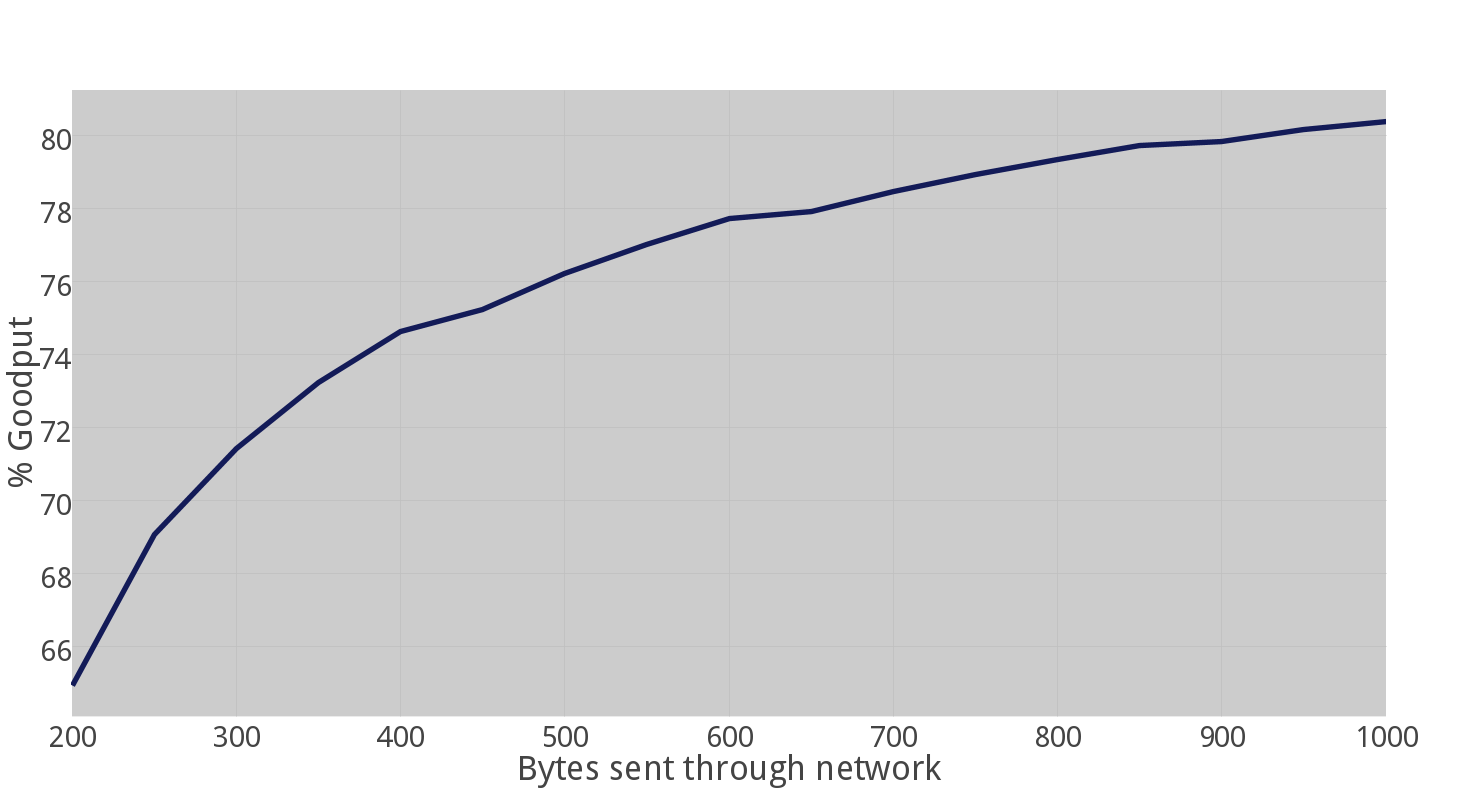
\includegraphics[scale=1.0]{NON_200toKplotx09_thickerLineGRAY.png}    
    \caption{NON 200-1000 bytes}
    \label{fig:NON200-kb}
\end{figure}



%\begin{figure}[ht]
%    \centering
%    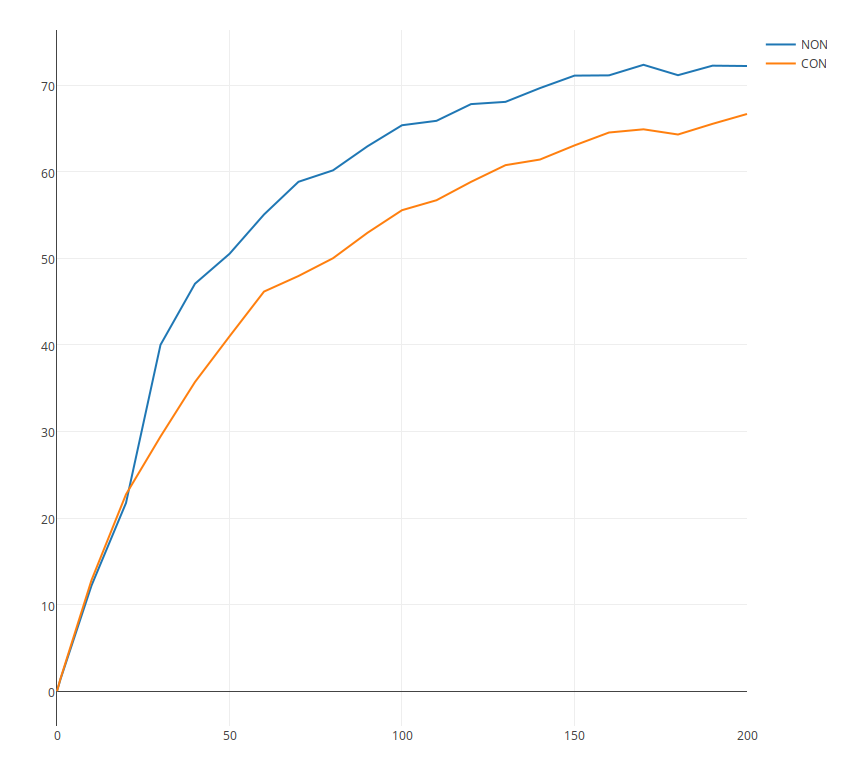
\includegraphics[scale=0.45]{CONvsNON1.png}    
%    \caption{CON vs NON}
%    \label{fig:CONvsNON}
%\end{figure}





%\begin{figure}[ht]
%    \centering
%    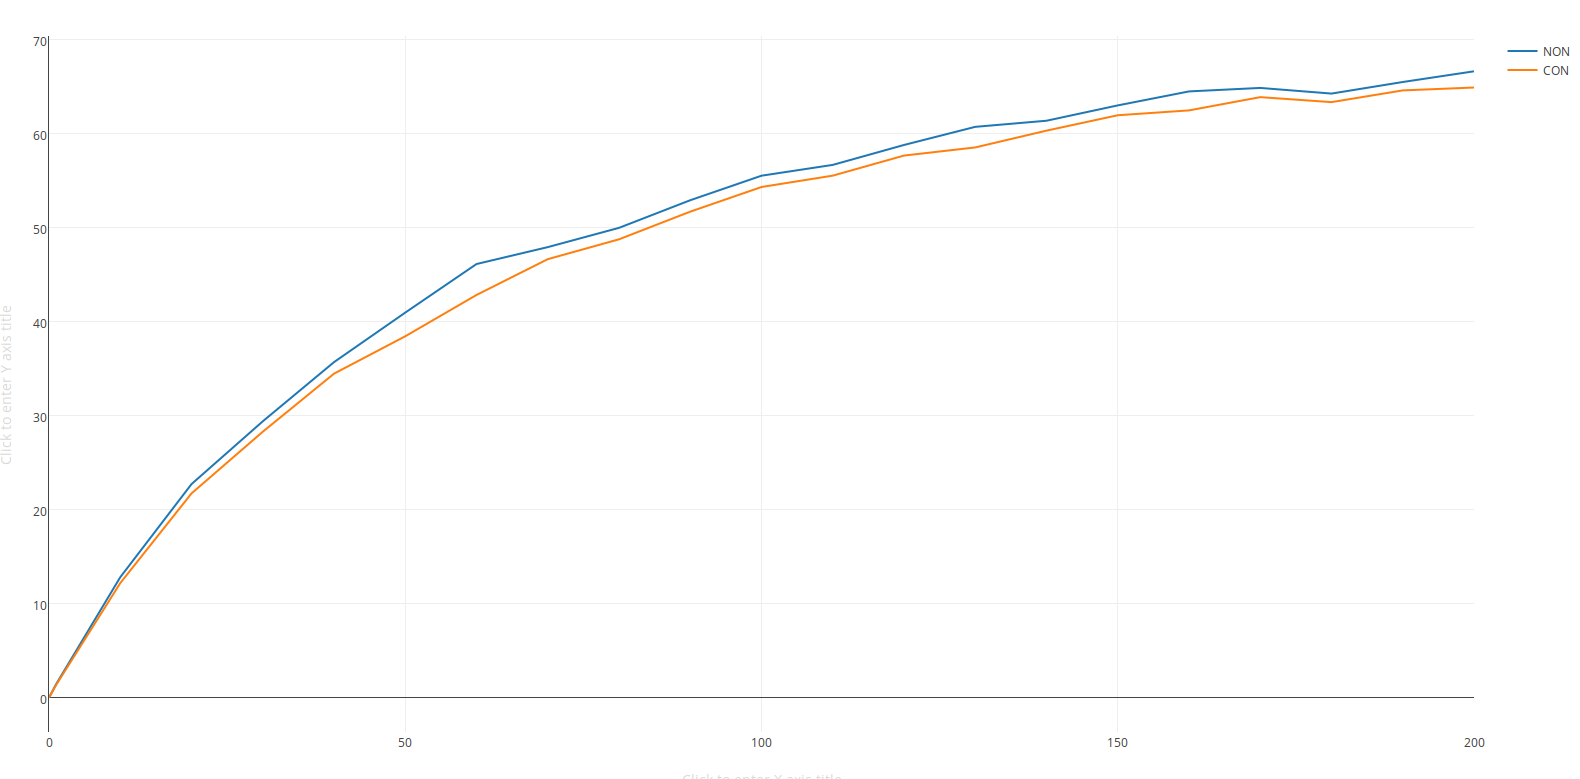
\includegraphics[scale=0.25]{CONvsNON0-200_2.png}    
%    \caption{CON vs NON 0-200 bytes number 2}
%    \label{fig:CONvsNON0-200}
%\end{figure}




\subsection{Discussion}

\section{Comparison}



\begin{figure}[ht]
    \centering
    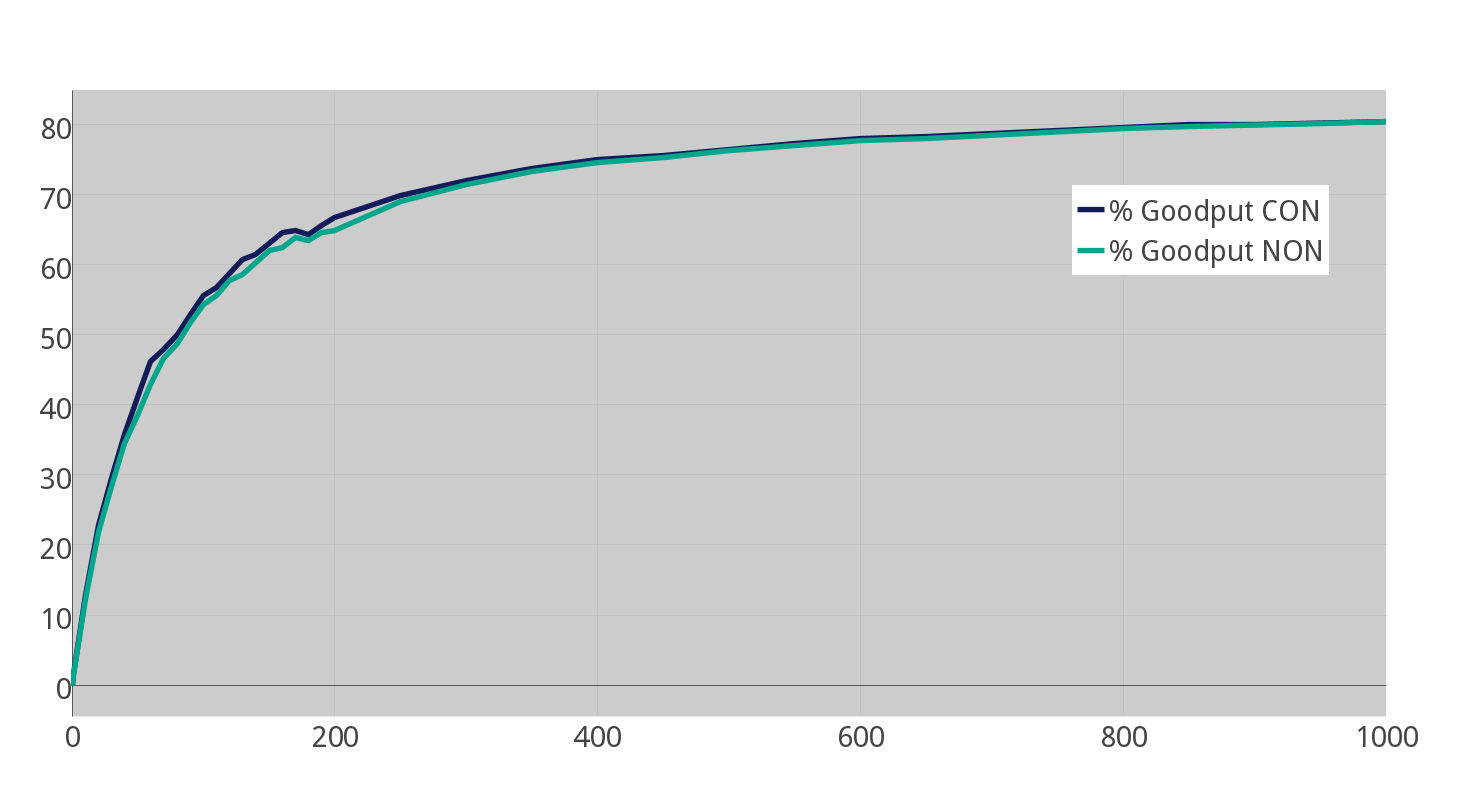
\includegraphics[scale=1.0]{CONvsNONplot_0-k_thickerGRAY.png}    
    \caption{CON vs NON 0-1000 bytes}
    \label{fig:CONvsNON0-1000}
\end{figure}

\begin{figure}[ht]
    \centering
    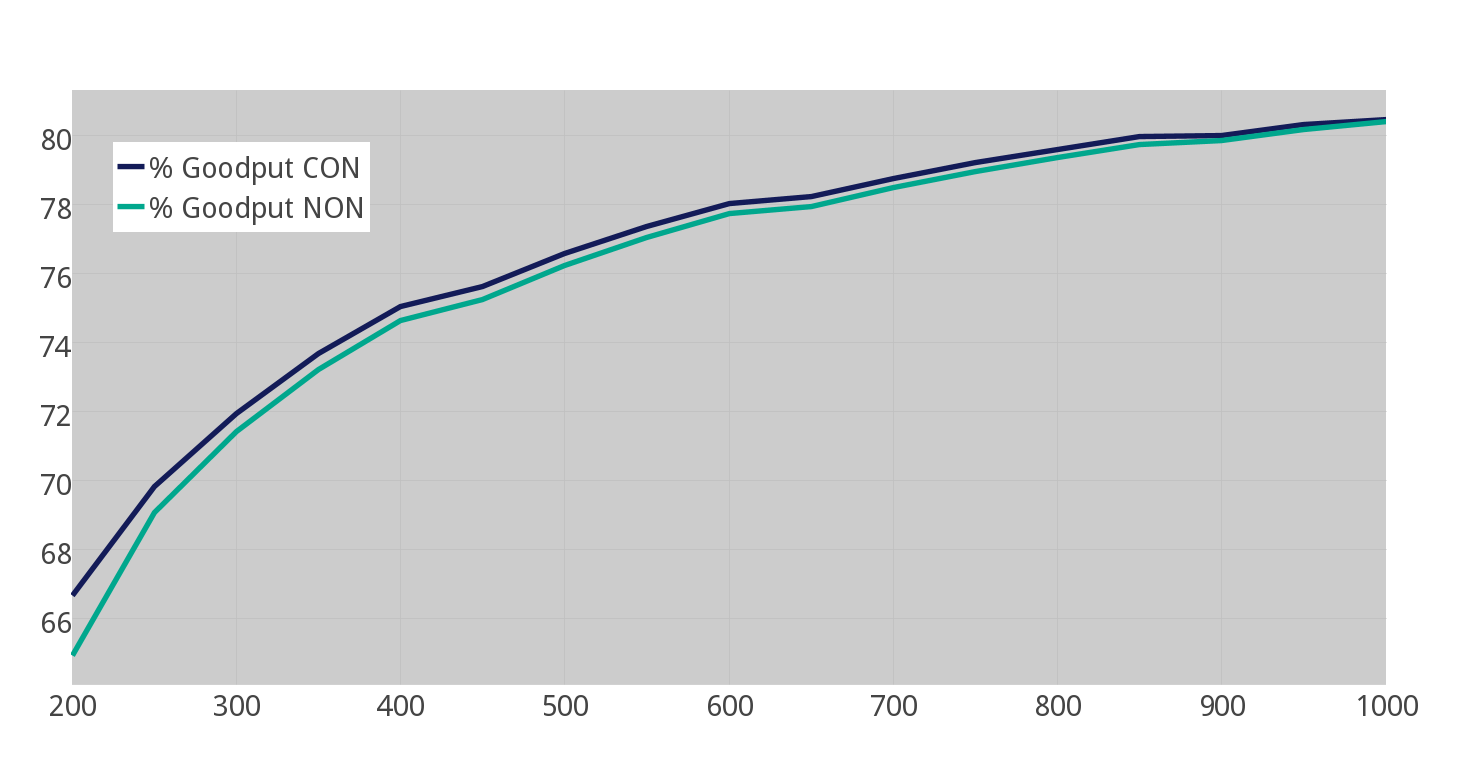
\includegraphics[scale=1.0]{CONvsNONplot_200-k_thickerGRAY.png}    
    \caption{CON vs NON 200-1000 bytes}
    \label{fig:CONvsNON200-1000}
\end{figure}

\subsection{Goodput per time interval}

Previous sections in this chapter has shown the percentage of bytes sent through that has been goodput, useful data, compared to the total amount of bytes. This is a good overview of how the protocols are able to exploit the network, and tells a lot about the different protocols. In a real world scenario however, the actual \textit{throughput per time} would be more relevant, since this tells how much data can be transported for every second.

\gls{coap} \gls{con} and \gls{non} has been compared in this thesis, but in the system build \gls{non} was quite unstable at high transfer rates, as explained in chapter \ref{chp:architecture}.1. Because of this, \gls{con} seems like a better solution only considering the number of bytes transferred per second. As it turns out, this depends. 

As seen in Table \todo{insert table}, this might be a too early conclusion.

The table shows timestamps of packets received on the Raspberry Pi, sent with both \gls{con} and \gls{non}. Packets was captured with Wireshark, and the timestamp is created by Wireshark on the form \textit{number of seconds since start of capture}. The first value for each packet size in the table therefore approximately notes the number of seconds from the connection starts until the first packet containing useful data has arrived \footnote{values far off from the expected results due to e.g. connection issues have been excluded in calculations }. The first thing that is noticeable here is the big difference before useful data can be received. Equation \ref{averageStartTimeCON} shows the calculations of average start time on \gls{con}, which is a lot higher than for \gls{non} shown in equation \ref{averageStartTimeNON}. The main reason for this is that the \gls{non} needs to have a connection establishment using \gls{con} packets with \glspl{ack} without data before \gls{non} packets can be transferred. In addition severe connection issues was experienced in a much higher grade using \gls{non} than \gls{con}, especially for packets larger than 500 bytes, as shown in table \todo{Refer to table}.  


\begin{equation} \label{averageStartTimeCON}
     \frac{3.4677+2.2425+4.0885+5.2941+3.3297+1.3398+4.6184+3.257+3.4062}{9} \approx 3.4493
\end{equation}


\begin{equation} \label{averageStartTimeNON}
	\frac{10.1609+10.0567+9.4627+8.5798+28.3489+29.069}{6} \approx 15.9463
\end{equation}

Figure \todo{Tegn graf om hvor mange pakker som kan sendes per sekund} 

\todo{Tegn graf om hvor lang tid det tar aa sende x andtall pakker, feks 13 eller 15?}





%\section{BLE}


\section{Time spent in network}

The previous tests shows 



Calcumate time for \gls{coap} \gls{non}, 700 bytes sent:

\begin{equation}
    ((55.9578-54.7750)+(57.1476-55.9578)+(58.3379-57.1476))/3 = 1.1876
\end{equation}

 	0.1876/3 = 0.0625


\section{Quantity test}

This section will show a test of several nRF52 devices connected to the same Pi at the same time, to ensure stability and performance in the network. Even though this puts more pressure on both the network and the Pi, it is not expected to be considerably noticed in the transportation of packets. 


\todo{Do measurements of several nRF52s. Write new python script to gather data from all of these. Add this to the Appendix}



\chapter{Discussion}
\label{chp:dataAnalysis}

\section{Set up network}

\noindent \textbf{O.1: Build a star network of microcontrollers}

\noindent  This objective was fulfilled by using the Raspberry Pi as a central node and nRF52s as end nodes. Central points in the solution was the use of a version of Linux \gls{os} with pre-configured kernel of version 4.15 or later on the \gls{Raspberry Pi}. In addition it was important to understand how prefix in \gls{ipv6} works, and how this can be used to identify a device connected using \gls{ble}. In this solution the end nodes with \glspl{nRF52} works as servers, while the central Raspberry Pi works as a client requesting services from these servers. 


\noindent \textbf{R.1: Which transport protocols are suitable for such a system?}

\noindent \gls{ble} was chosen over ANT, as explained in chapter \ref{chp:background}.2.3. Bluetooth is a widely used technology that is very interesting in an \gls{iot} setting, and was therefore the obvious choice in this network. The \gls{ble} version of Bluetooth is designed to use a minimal amount of energy and still be reliable and fast, which is central criteria in the testbit. As a result of this \gls{6lowpan} also seemed like a suitable communication protocol, both because it is made to work together with \gls{ble}, and because it is an up an coming technology that is assumed to be more and more used in the coming years. \textit{Zigbee} and \textit{Zensys} were the main other options, which did not seem as fit in this case mostly because of different solutions in routing. In the application layer the two main choices was between \gls{coap} and \gls{mqtt}. Because of time restrictions \gls{coap} was chosen to be studied in depth in this thesis. 

\newpage


\section{Gather sensor data}

\noindent\textbf{O.2: Connect sensors to the end-nodes to collect data}

\noindent This objective was partially fulfilled. An accelerometer was connected to two of the end nodes in the network, with the goal of gathering vibration data to be sent through the network. Problems occurred when getting the accelerometer to communicate properly with the end node, meaning that it was possible to gather acceleration data, but not as frequently as expected. Getting reliable vibration data was therefore not possible. Due to these problems, in addition to the main scope of this thesis, it was decided to measure the different aspects of the network with simulated data instead of real world vibration data. This would eliminate the possibility of errors due to problems with the sensor, letting this objective to be completed later by future work. 

\noindent Even though this objective was not fully completed, related coding was done on the \gls{nRF52} to be able to initialize and use the accelerometer connected. This code can be useful for later projects in future works, and central aspects from the code will therefore be included in appendix \ref{chp:appendixc}.  



\section{Send data through network}

\noindent\textbf{O.3: Gather information of the data sent through the network}

\noindent This object was fulfilled by using both Python scripts and Wireshark on the \gls{Raspberry Pi} to measure the packets sent through the network. Different Python scripts were used to get data from the servers, save data locally after receiving, drawing graphs directly to represent the data, or to forward the data to another device or online storage facility. The most central of these code samples can be seen in appendix \ref{chp:appendix}. Wireshark was used to monitor the live capture of packets, and to manually do a detailed analysis of how packets where fragmented differently in the different scenarios. 

\noindent\textbf{R.2: What are the main limitations concerning transporting data?}

\noindent Already in the first tests of \gls{rtt} shown in chapter \ref{chp:measurements2}.1.1, it became clear that one of the major limitations in this network would be the initial transfer speed. This was not expected, and was not included as one of the main objectives in this thesis, which concentrates more on analysing and discussing the data sent through the network, and transport protocols used. It is assumed that this is a problem in a lower level of the protocol stack, and will be left for future work to solve. Other than this, limitations regarding network stability were found. Several of the tested solutions were not able to transfer data at all, or only for a very short period (< 20 seconds). When a stable solution was found, the link could be open as long as needed. Successful tests have been running for several days. During these tests it was discovered that the message ID implemented in \gls{coap} uses an 16 bit counter. After 65536 messages have been sent the counter will be reset, and changed to 18 bits. This did not affect the performance in this system, and will most likely not be a problem in other systems as well. Other limitations discussed in detail in this thesis was the frequency data can be sent through the network, unstable connections when the \gls{payload} gets too big, device failure at runtime then the \gls{payload} gets too big and power consumption increases. 

\noindent\textbf{R.3: Are the microcontrollers powerful enough to gather data this frequently?}

\noindent To gather detailed acceleration data to be analysed in another node of the network, we assume that a measuring frequency of 1MHz is needed. The maximum achieved in this system was to call a method from the main loop 11 times every second, and then read a measured values from the accelerometer 150 times for each of these 11 method calls. This adds up to 1650 measuring points every second in a best case scenario. Yes, this is fast enough to gather data, even though problems explained in chapter \ref{chp:architecture} means this practical experiment will be left for future work in this thesis. The programming code referred to here can be seen in appendix \ref{chp:appendixc}. 

 %\todo{Why 1MHz?}

\section{Analyse data}

\noindent\textbf{O.4: Analyse and discuss the gathered information}

\noindent This object was fulfilled by analysing the data by printing out table and plotting graphs. Using basic tools like this it was possible to document both the differences and similarities in the different protocols tested in this thesis. The results where presented and discussed in detail in chapter \ref{chp:measurements2}.

\noindent\textbf{R.4: Could data analysis be done in the end nodes in this network?}

\noindent Referring to the result from research question R.3. The maximum capacity of the \gls{microcontroller} is needed to capture acceleration data from the accelerometer, get the desired quality of the data, and forward this to a central node. The end nodes were running on battery power. To do even more calculations in these nodes will not be preferable in this network. This will be possible if the node is one of many nodes in a complete network, where every node gets some time of sleep between every measurement. Even here it is probably not a good idea, concerning the use of batteries. The answer is therefore no, more detailed analysing and representation of the data should be done in a central node with more computational power and better access to power sources. 
% \todo{Remove parts about battery power?}

\newpage
\subsection{Measurements}

%\todo{Write more about problems, too slow network throughput, to unstable. }

\noindent As a summary of the measurements presented in this thesis, the positive and negative aspects of the two versions of \gls{coap} that have been tested will be be directly compared to get a more clear understanding of the differences, advantages and disadvantages.


\begin{table}[H]
\centering
\caption{Comparison of CON and NON}
\label{ComparisonTable}
\begin{tabular}{|c|c|c|c|l}
\cline{1-4}
\textbf{Case}                                                                                                                               & \textbf{CON}               & \textbf{NON}               & \textbf{Comments}                                                                                                                       &  \\ \cline{1-4}
Need of ACKs                                                                                                                                & Yes                        &  \textbf{No}                         & \begin{tabular}[c]{@{}c@{}}Accational connection \\ test at 16+7+7 bytes\\  in both cases\end{tabular}                                  &  \\ \cline{1-4}
\begin{tabular}[c]{@{}c@{}}Minimum number of \\ bytes needed for \\ empty CoAP message\end{tabular}                                         & 74+104                     &\textbf{76}                         &                                                                                                                                         &  \\ \cline{1-4}
\begin{tabular}[c]{@{}c@{}}Fastest for payload \\ \textless 500 byte\end{tabular}                                                           & \textbf{X}                          &                            & \begin{tabular}[c]{@{}c@{}}Almost 3x faster\\ payload \textless 10 byte\end{tabular}                                                    &  \\ \cline{1-4}
\begin{tabular}[c]{@{}c@{}}Fastest for payload \\ \textgreater 500 byte\end{tabular}                                                        &                            & \textbf{X}                          & \begin{tabular}[c]{@{}c@{}}On average 0,2 s faster\\ for payload \textgreater 600 byte\end{tabular}                                     &  \\ \cline{1-4}
\begin{tabular}[c]{@{}c@{}}Average time {[}seconds{]} \\ to send 200 bytes payload\end{tabular}                                             & \textbf{0,66}                       & 1,00                       &                                                                                                                                         &  \\ \cline{1-4}
\begin{tabular}[c]{@{}c@{}}Average time {[}seconds{]}\\  to send 700 bytes payload\end{tabular}                                             & 1,32                       & \textbf{1,21}                       &                                                                                                                                         &  \\ \cline{1-4}
\begin{tabular}[c]{@{}c@{}}Highest measured \\ goodput {[}bytes{]} \\ per second\end{tabular}                                               & \textbf{608}                        & \textbf{611}                        &                                                                                                                                         &  \\ \cline{1-4}
\begin{tabular}[c]{@{}c@{}}Overall best stability\\ in the network\end{tabular}                                                             & \textbf{X}                          &                            &                                                                                                                                         &  \\ \cline{1-4}
\begin{tabular}[c]{@{}c@{}}Calculated lowest \\ power concumption\end{tabular}                                                              &                            & \textbf{X}                          &                                                                                                                                         &  \\ \cline{1-4}
\multicolumn{1}{|l|}{\begin{tabular}[c]{@{}l@{}}\% payload of all packets\\ sent through network\\ (in case of 500 byte sent)\end{tabular}} & \multicolumn{1}{l|}{63,21} & \multicolumn{1}{l|}{\textbf{83,56}} & \multicolumn{1}{l|}{\begin{tabular}[c]{@{}l@{}}On average 20\% more \\ efficient in the number \\ of packet sent in total\end{tabular}} &  \\ \cline{1-4}
\end{tabular}
\end{table}

\newpage
\noindent Table \ref{ComparisonTable} shows a summary of the main results found in the comparison of \gls{coap} \gls{con} and \gls{non} in the network presented in this thesis. Results from the table shows that in 7 of the 10 cases presented, \gls{non} shows the best results.  This should still not be a final result without discussion. As discussed in chapter \ref{chp:measurements2}, \gls{non} has been considerably more unstable than \gls{con} during the test period. It was not possible to get a stable connection when sending more frequently than once every second, and the connection became unstable if the payload was greater than 800 bytes. As a conclusion from this table it is clear to say that \gls{non} works best if the conditions are right, sending data every second with a payload between 500 and 700 bytes. In other cases than this, \gls{con} works better in the practical experiments presented.

\noindent Looking at the network in general using \gls{coap}, the slowest transfer time is 2 seconds to transfer 1 kB of \gls{payload}. This is considered very slow through a network like this. \gls{ble} has a given \gls{mtu} of 1 MB per second, far beyond what has been achieved in the tests presented here. The highest achieved \gls{goodput} was about 500 bytes/second, or 1/2 MB/second. \gls{ble} is therefore not the main limitation in the network. \gls{coap} creates the messages sent, but should not influence on the network throughput, if not the action of making the packets in the end node is the limitation. \gls{6lowpan} is only used as a way of transporting data in the network, and will therefore not affect the throughput in the system. Final possibility is that the limitation is in the computational power of one of the devices communicating with each other. In this case it makes sense to assume the \gls{nRF52}, both since this is the sending part of the network needing to process the data and construct the packets being sent, and because it has significantly less power capacity than the \gls{Raspberry Pi}.

\noindent This brings the question up for discussion if it is profitable to send data larger than 1 kB at all. If the sending rate keeps climbing at the same rate as measured here, with a rate of 1 second slower for every 500 bytes. As a comparison it will take 1000 seconds to transfer 500 kb, which is more than 15 minutes. 


\section{Ease of use}


\subsection{Raspberry Pi}

\noindent As a central device for the \glspl{microcontroller}, the \gls{Raspberry Pi} has worked great. There are several good options when it comes to choosing an \gls{os} that can be customised for a specific system, and several good guides that makes this a simple and fast small device for most end users. 


\subsection{nRF52}

\noindent The \gls{nRF52} requires a lot more experience both in programming and general understanding of computers to be used properly than the \gls{Raspberry Pi}. Online documentation is available and is usually very good, but also some times a bit confusing and messy. A great tool is the Nordic Semiconductor forum specially designed for questions regarding this and other Nordic devices\footnote{\url{https://devzone.nordicsemi.com}}. Example code is also provided by Nordic, to show how the device can be used with different technologies. This works as a starting point, but it is very time consuming and difficult for an end user without specific experience on this device to familiarize with how this code works, in order to change to something else instead. The example code used as an example in this thesis was not optimized for battery consumption, and as a result the small battery drained very fast during the testing. This is of course possible to optimize for an experienced user, but should be taken into account for the average end user of such a device in a complete system. 







\chapter{Conclusion and Future Work}
\label{chp:results}



\noindent In this thesis I have used \glspl{microcontroller}, sensors, \glspl{singleBoardComputer} and a stationary computer to build an \gls{iot} network. Using this network I have tested some of the choices a system developer can face when transporting data through the network, particularly emphasising Bluetooth Low Energy and 6LoWPAN. Central topics for discussion has been analysis of data with respect to network capacity, network exploitation, transfer rate and power usage. 

\noindent From the results presented concerning fragmentation of data, the thesis argues that neither in \gls{coap} \gls{con} or \gls{non} is fragmentation a major concern. Both the max size of 31 bytes of \gls{ble} packets and 270 bytes of \gls{6lowpan} packets was exceeded in the test, without having major affect on the percentage of \gls{payload} sent through the network compared to the total \gls{throughput}. This would otherwise have resulted in a more uneven slope of the graphs presented. 

\noindent In addition to this, the thesis has presented experiments to analyse and discuss the \gls{goodput} in the system. Results shows that \gls{coap} \gls{con} is faster for smaller \glspl{payload}, while \gls{non} if the \gls{payload} is bigger than 500 bytes. The highest \gls{goodput} achieved was 611 bytes/second, and overall the system needs almost 1 additional second for every 500 bytes of \gls{payload} being added. This is quite slow compared to the limitations of the different technologies used, and it is being discussed what can be the main reason for this. The author did not have the resources to investigate this in detail within the time frame, but it seems reasonable to assume that the limitation is not \gls{ble} or \gls{6lowpan}, but rather limitations in the computational power or wireless antennas of one of the devices used. 

\noindent The last experiment presented shows that \gls{non} require the least packets in best case, but also the most in worst case to transfer the same \gls{payload}. Despite this, \gls{non} most of the time manages to stay on best case, giving it the best \% payload of all packets sent at 500 bytes, with 83,56 \% compared to 63,21 \% in \gls{con}.

\noindent All results put together shows that both \gls{ble} and \gls{6lowpan} works in such a system, together with both versions of \gls{coap} tested. In some cases the network was stable and reliable, but there where also several limitations which lead to problems during the testing. Limited sending frequency, limited payloads and difficulties when connecting to other devices is the most central. Still I will say the network is a very interesting stating point to a more complex \gls{iot} system, that can definitely be used as a starting point for future projects. 


\section{Future Work}

\noindent This thesis does not have any direct previous works, but explains how to build a basic \gls{iot} system using devices of different size and limitations. The project has had a limited time frame, and naturally this leads to several possibilities concerning future works, both by adding other objectives and to complete the objective that was not fully completed in this thesis. 

\noindent A proposed future work is to build the network further both with \glspl{microcontroller} and computational power, as a direct addition to the system presented. The system can be expanded a lot both concerning bigger and smaller devices, for instance can several sensors be connected to the same \gls{microcontroller}, and several \glspl{microcontroller}, both \glspl{nRF52} and others, can be connected at the same time to get a more real world environment to test data. In the other end the system can be set up both to ask for computational power from a supercomputer or to automatically display the results on a web page on a database. It would then be possible create a more user friendly \gls{ui}, which would make it easier to test and analyse even bigger loads of data sent through the system. 


%\begin{figure}[ht]
%    \centering
%    \includegraphics[width=1.0\textwidth]{ArchitectureChapIntro1.png}    
%    \caption{Complete system architecture}
%    \label{fig:systemArchitectureFuture}
%\end{figure}





\renewcommand*{\bibname}{References}
\bibliographystyle{chicago} %alpha
\bibliography{main}

%% Uncomment the following if you have any appendix
 \appendix
 \addtocontents{toc}{%
  \protect\vspace{1em}% 
  \protect\noindent \bfseries \appendixtocname\protect\par
  \protect\vspace{-.5em}%
 }
 \renewcommand{\appendix}{\appendixname}
%% include below possible appendices (chapters)
\chapter{Appendix A}
\label{chp:appendix}

Appendix A contains samples of programming code used to gather and transfer data in the \gls{iot} system described in this thesis. 

\section{Python programming scripts}

This first example is the most simple, using \textit{GET} commands to get the measured values from \gls{coap} \gls{con}. All the python scripts uses example code from Nordic Semiconductor in 

\begin{lstlisting}[language=Python]
import asyncio
from aiocoap import *

SERVER_ADDR = '2001::2AF:B7FF:FEB6:1494'
SERVER_PORT = '5683'
SERVER_URI  = 'coap://[' + SERVER_ADDR + ']:' + SERVER_PORT

@asyncio.coroutine
def main():
	protocol = yield from Context.create_client_context()
	sequence_number = 1
	number_of_measurements = 200
	while sequence_number < number_of_measurements:
		request_acceleration = Message(code=GET)
		request_acceleration.set_request_uri(SERVER_URI + '/lights/led3')
		response = yield from protocol.request(request_acceleration).response
		print('Acceleration'+str(sequence_number)+': %s Response Code: %s\n'%(response.payload, response.code))		
		sequence_number += 1

if __name__ == "__main__":
	asyncio.get_event_loop().run_until_complete(main())

\end{lstlisting}

\newpage

This script was written to get observable values stored in a local file. 

% Observable to file
\begin{lstlisting}[language=Python]
import asyncio
from aiocoap import *

#SERVER_ADDR = '2001::211:64ff:fea5:8542'
SERVER_ADDR = '2001::2e6:6aff:fe64:54dd'
#SERVER_ADDR = '2001::2af:b7ff:feb6:1494'
SERVER_PORT = '5683'
SERVER_URI  = 'coap://[' + SERVER_ADDR + ']:' + SERVER_PORT

responseList = []
def observe_handle(response):
	f = open('/home/sindre/Desktop/desktopAccelValues', 'a')
	if response.code.is_successful(): 	
		responseList = bytes.decode(response.payload) 
		for i in range(0, (len(responseList))):
			f.write((str(responseList[i]) + ' '))
		f.write(responseList)		
		f.write('\n')
		print("Written to file!")
	else:
		print('Error code %s' % response.code)
	f.close()
@asyncio.coroutine
def main():
    protocol = yield from Context.create_client_context()
    request = Message(code=GET)
    request.set_request_uri(SERVER_URI  + '/lights/led3')
    request.opt.observe = 0
    observation_is_over = asyncio.Future()
    try:
        requester = protocol.request(request)
        requester.observation.register_callback(observe_handle)
        response = yield from requester.response
        exit_reason = yield from observation_is_over
        print('Observation is over: %r' % exit_reason)
    finally:
        if not requester.response.done():
            requester.response.cancel()
        if not requester.observation.cancelled:
            requester.observation.cancel()

if __name__ == "__main__":
    asyncio.get_event_loop().run_until_complete(main())


\end{lstlisting}

This example is to get observable measurements directly displayed in a graph: 
% Observable to plot
\begin{lstlisting}[language=Python]
import asyncio
from aiocoap import *
import matplotlib.pyplot as plt

#SERVER_ADDR = '2001::211:64ff:fea5:8542'
SERVER_ADDR = '2001::2e6:6aff:fe64:54dd'
#SERVER_ADDR = '2001::2af:b7ff:feb6:1494'

SERVER_PORT = '5683'
SERVER_URI  = 'coap://[' + SERVER_ADDR + ']:' + SERVER_PORT

responseList = []
drawValuesList = []

def observe_handle(response):
	if response.code.is_successful(): 	
		responseList = bytes.decode(response.payload) 	
		print(responseList)

		for i in range (0,len(responseList)):
			drawValuesListappend(int(responseList[i]))
		plt.plot(drawValuesList)
		plt.xlabel('Measurement number')
		plt.ylabel('Acceleration values')
		plt.show()	
		
	else:
		print('Error code %s' % response.code)
@asyncio.coroutine

def main():
    protocol = yield from Context.create_client_context()
    request = Message(code=GET)
    request.set_request_uri(SERVER_URI  + '/lights/led3')
    request.opt.observe = 0
    observation_is_over = asyncio.Future()
    try:
        requester = protocol.request(request)
        requester.observation.register_callback(observe_handle)
        response = yield from requester.response
        exit_reason = yield from observation_is_over
        print('Observation is over: %r' % exit_reason)
    finally:
        if not requester.response.done():
            requester.response.cancel()
        if not requester.observation.cancelled:
            requester.observation.cancel()

if __name__ == "__main__":
    asyncio.get_event_loop().run_until_complete(main())

\end{lstlisting}





\chapter{Appendix B}
\label{chp:appendixb}

Appendix B contains screenshots and detailed figures from the measurements done in the network built in this thesis. 



\begin{center}
 \begin{tabular}{||c c c c||} 
 \hline
 Goodput & Throughput & NON packet size & (Goodput/Throughput)*100 \\ [0.5ex] 
 \hline\hline
 0 & 71 & 76 & 0 \\ 
 \hline
 1 & 73 & 78 & 1,37 \\
 \hline
 10 & 82 & 87 & 12,20 \\
 \hline
 20 & 92 & 97 & 21,74 \\
  \hline
 30 & 75 & 107 & 30,0 \\
  \hline
 40 & 85 & 117 & 47,06 \\
  \hline
 50 & 99 & 127 & 50,51 \\
  \hline
 60 & 109 & 137 & 55,05 \\
  \hline
 70 & 119 & 147 & 58,82 \\
  \hline
 80 & 133 & 157 & 60,15 \\
  \hline
 90 & 143 & 167 & 62,94 \\
 \hline
 100 & 153 & 177 & 65,36 \\
 \hline
 110 & 167 & 187 & 65,87 \\
 \hline
 120 & 177 & 197 & 67,80 \\
 \hline
 130 & 191 & 207 & 68,06 \\
 \hline
 140 & 207 & 217 & 69,65 \\
 \hline
 150 & 211 & 227 & 71,09 \\
 \hline
 160 & 225 & 237 & 71,11 \\
 \hline
 170 & 235 & 247 & 72,34 \\
 \hline
 180 & 253 & 257 & 71,15 \\
 \hline
 190 & 263 & 267 & 72,24 \\
 \hline
 200 & 277 & 277 & 72,20 \\ [1ex] 
 \hline
\end{tabular}
%\caption{Measurements, BLE, constant length}
\label{table:1}
\end{center}

\end{document} 
